\documentclass[10pt]{beamer}
\usepackage{amsmath}
\usepackage{mathtools}
\usepackage{multimedia}
\usepackage{hyperref}
\usefonttheme{professionalfonts} % using non standard fonts for beamer
\usefonttheme{serif} % default family is serif
%\documentclass[12pt]{beamerthemeSam.sty}
\usepackage{epsf}
%\usepackage{pstricks}
%\usepackage[orientation=portrait,size=A4]{beamerposter}
\geometry{paperwidth=162mm,paperheight=108mm}
%DT favorite definitions
\def\LL{\left\langle}	% left angle bracket
\def\RR{\right\rangle}	% right angle bracket
\def\LP{\left(}		% left parenthesis
\def\RP{\right)}	% right parenthesis
\def\LB{\left\{}	% left curly bracket
\def\RB{\right\}}	% right curly bracket
\def\PAR#1#2{ {{\partial #1}\over{\partial #2}} }
\def\PARTWO#1#2{ {{\partial^2 #1}\over{\partial #2}^2} }
\def\PARTWOMIX#1#2#3{ {{\partial^2 #1}\over{\partial #2 \partial #3}} }

\def\rightpartial{{\overrightarrow\partial}}
\def\leftpartial{{\overleftarrow\partial}}
\def\diffpartial{\buildrel\leftrightarrow\over\partial}

\def\BS{\bigskip}
\def\BC{\begin{center}}
\def\EC{\end{center}}
\def\BCC{\begin{columns}}
\def\ECC{\end{columns}}
\def\HC{\column{0.5\textwidth}}
\def\BI{\begin{itemize}}
\def\EI{\end{itemize}}
\def\BE{\begin{displaymath}}
\def\EE{\end{displaymath}}
\def\BEA{\begin{eqnarray*}}
\def\EEA{\end{eqnarray*}}
\def\BNEA{\begin{eqnarray}}
\def\ENEA{\end{eqnarray}}
\def\EL{\nonumber\\}


\newcommand{\etal}{{\it et al.}}
\newcommand{\gbeta}{6/g^2}
\newcommand{\la}[1]{\label{#1}}
\newcommand{\ie}{{\em i.e.\ }}
\newcommand{\eg}{{\em e.\,g.\ }}
\newcommand{\cf}{cf.\ }
\newcommand{\etc}{etc.\ }
\newcommand{\atantwo}{{\rm atan2}}
\newcommand{\Tr}{{\rm Tr}}
\newcommand{\dt}{\Delta t}
\newcommand{\op}{{\cal O}}
\newcommand{\msbar}{{\overline{\rm MS}}}
\def\chpt{\raise0.4ex\hbox{$\chi$}PT}
\def\schpt{S\raise0.4ex\hbox{$\chi$}PT}
\def\MeV{{\rm Me\!V}}
\def\GeV{{\rm Ge\!V}}

%AB: my color definitions
%\definecolor{mygarnet}{rgb}{0.445,0.184,0.215}
%\definecolor{mygold}{rgb}{0.848,0.848,0.098}
%\definecolor{myg2g}{rgb}{0.647,0.316,0.157}
\definecolor{A}{rgb}{1.0,0.3,0.3}
\definecolor{B}{rgb}{0.0,1.0,0.0}
\definecolor{C}{rgb}{1.0,1.0,0.0}
\definecolor{D}{rgb}{0.5,0.5,1.0}
\definecolor{E}{rgb}{0.7,0.7,0.7}
\definecolor{abtitlecolor}{rgb}{1.0,1.0,1.0}
\definecolor{absecondarycolor}{rgb}{0.0,0.416,0.804}
\definecolor{abprimarycolor}{rgb}{1.0,0.686,0.0}
\definecolor{Red}           {cmyk}{0,1,1,0}
\definecolor{Grey}          {cmyk}{.7,.7,.7,0}
\definecolor{Blue}          {cmyk}{1,1,0,0}
\definecolor{Green}         {cmyk}{1,0,1,0}
\definecolor{Brown}         {cmyk}{0,0.81,1,0.60}
\definecolor{Silver}        {rgb}{0.95,0.9,1.0}
\definecolor{Sky}           {rgb}{0.07,0.0,0.2}
\definecolor{Darkbrown}     {rgb}{0.4,0.3,0.2}
\definecolor{40Gray}        {rgb}{0.4,0.4,0.5}
\usetheme{Madrid}


\setbeamercolor{normal text}{fg=Silver,bg=Sky}

%AB: redefinition of beamer colors
%\setbeamercolor{palette tertiary}{fg=white,bg=mygarnet}
%\setbeamercolor{palette secondary}{fg=white,bg=myg2g}
%\setbeamercolor{palette primary}{fg=black,bg=mygold}
\setbeamercolor{title}{fg=abtitlecolor}
\setbeamercolor{frametitle}{fg=abtitlecolor}
\setbeamercolor{palette tertiary}{fg=white,bg=Darkbrown}
\setbeamercolor{palette secondary}{fg=white,bg=absecondarycolor}
\setbeamercolor{palette primary}{fg=white,bg=40Gray}
\setbeamercolor{structure}{fg=abtitlecolor}

\setbeamerfont{section in toc}{series=\bfseries}

%AB: remove navigation icons
\title[Telescopes]{
	\textbf {Telescopes}}

\author [Walter Freeman]{Syracuse University Physics\\Walter Freeman}

\date{\today}

\begin{document}

\frame{\titlepage}

\frame{
	\Large
	
	How did we get from here ... 
	\begin{flushright}
		... all the way to here?
	\end{flushright}

\begin{minipage}{0.49\textwidth}
	\BC
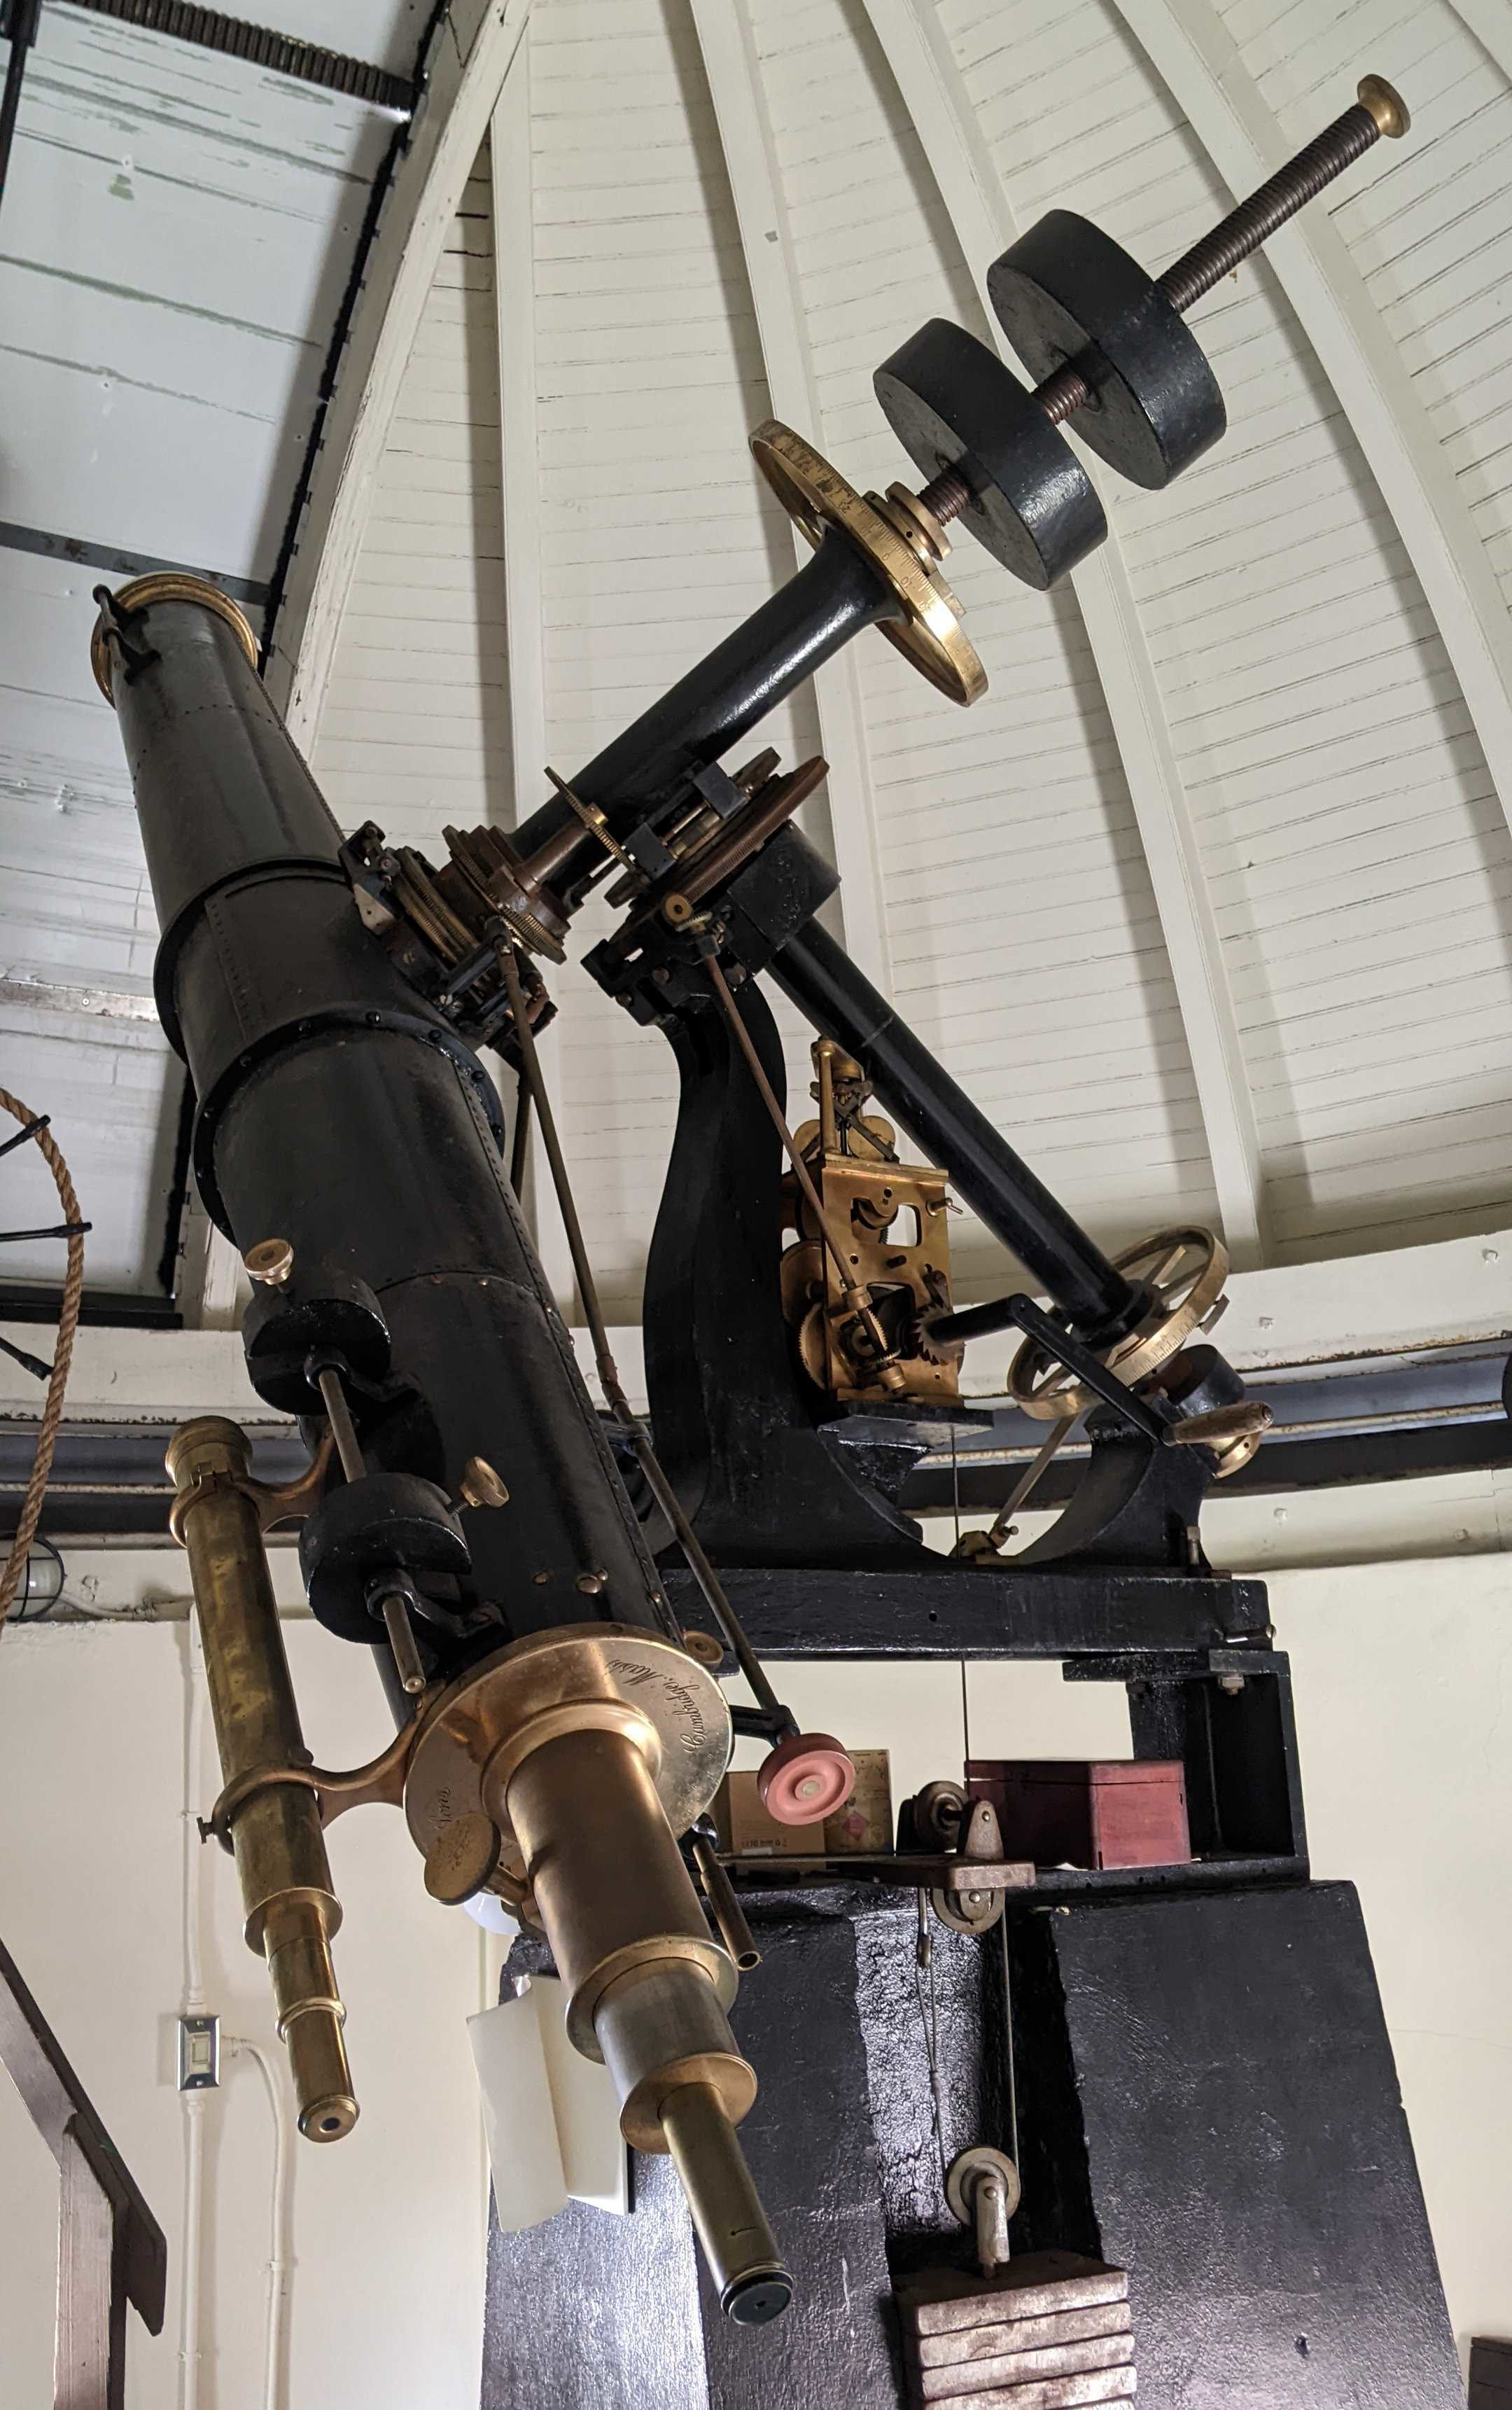
\includegraphics[width=0.7\textwidth]{holden.jpg} 

\scriptsize Telescope in Holden Observatory, Syracuse University (1887)
\EC
\end{minipage}
\begin{minipage}{0.49\textwidth}
\BC
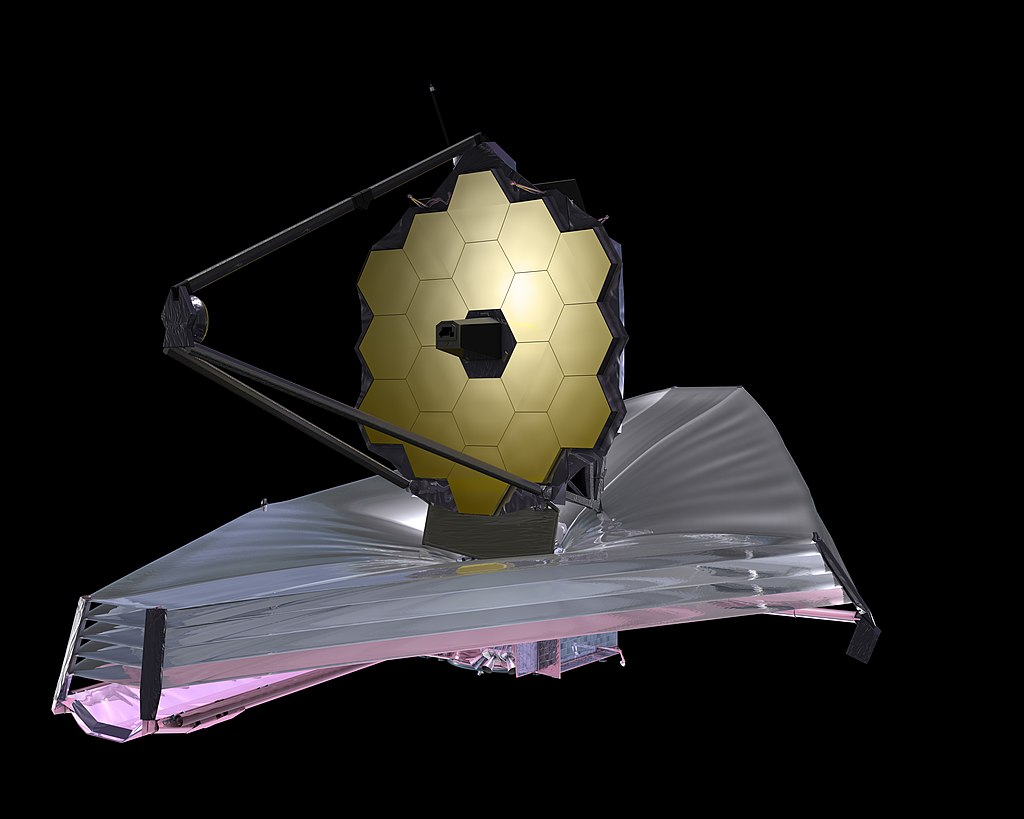
\includegraphics[width=0.9\textwidth]{jwst.jpg}
\vfill
\scriptsize Illustration, James Webb Space Telescope \\(NASA / ESA / CSA)
\EC
\end{minipage}
}

\frame{\frametitle{\bf Outline}
	\large
	
	\begin{enumerate}
		\item The Holden telescope: What is a telescope, anyway?
%		\BI
%		\item A machine to see small things
%		\item A machine to see faint things
%		\pause
%		\item A machine that gathers light
%		\EI
		
		\vspace{1em}\pause
		
		\item In pursuit of size: why is bigger better?
%		\BI
%		\item Big telescopes can see {\it fainter} things
%		\item Big telescopes can see smaller things
%		\pause
%		\item Mirrors are better than lenses!
%		\EI

		\vspace{1em}\pause
		
		\item Problems from the atmosphere
%		\BI
%		\item The atmosphere is in the way
%		\item Dry, still air is better than damp, turbulent air
%		\EI
		
				\vspace{1em}
		
		\item Somewhere over the rainbow: the spectroscopic revolution
%		\BI
%		\item There are many aspects of color our eyes can't see
%		\item These details tell us profound things about objects in space
%		\pause
%		\item ... and we have trouble seeing them through the atmosphere!
%		\EI
%		
	
				\vspace{1em}

\item To space: the Hubble Space Telescope
%\BI
%\item Why put a telescope in space?
%\item Limits of Hubble
%\pause
%\item It's small and warm
%\EI

\vspace{1em}


\vspace{1em}

\item The Webb telescope: solving problems in infrared astronomy
%\BI
%\item It's big
%\item It's in space
%\item It's cold
%\EI

\vspace{1em}
\item JWST scientific goals and images



\end{enumerate}
}

\frame{\frametitle{\bf What is a telescope?}
	
\BC \Large	A telescope is just a really big eyeball! \EC

\large Use a big lens or mirror to gather light and focus it to form an image.

	
	\BCC
	\HC
	
	\BS
	\BC
	It's just like an eyeball...\EC
		\HC
	\BC
	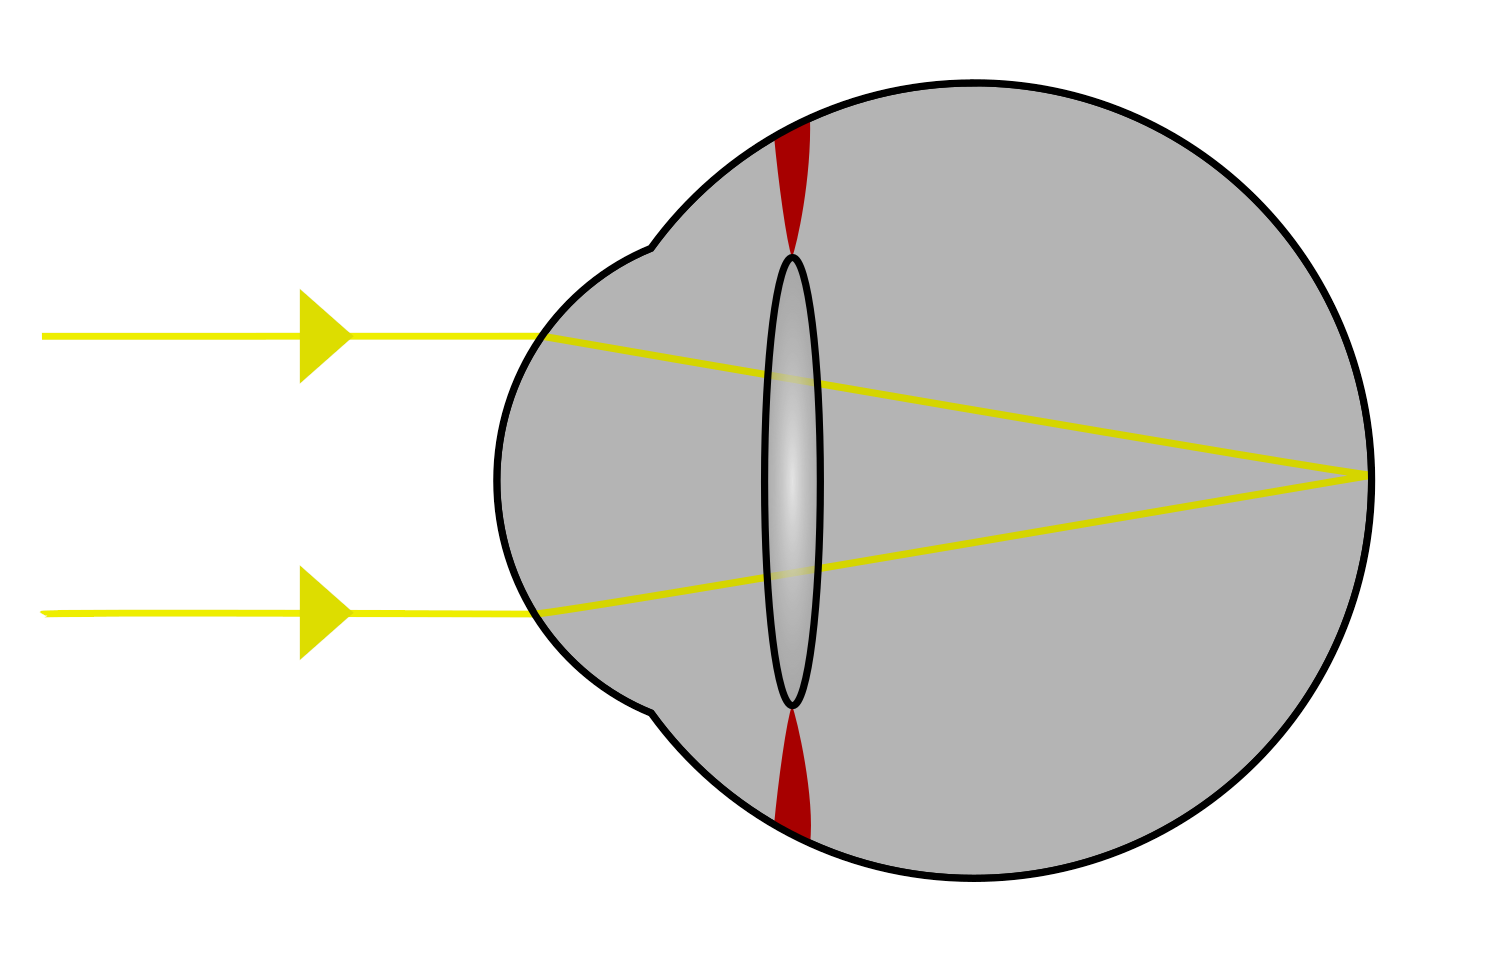
\includegraphics[width=0.5\textwidth]{eyeball.png}
	\EC
	\ECC
	

	\BCC
	\HC
	\BC
	... or a camera lens:\EC
	
	\normalsize
	
	\BI
	\item Using a shorter focal length lens produces a less magnified image
	\item Using a longer focal length lens produces a more magnified image
	\EI
	
	\HC
	
	

	
	\ECC
	
}

	\frame{\frametitle{\bf Eyepieces}
		
		\BC \Large These images can be too small to see well with the eye! 
		
		\BS 
		
		\large This makes sense if you compare a telescope to an eyeball:
		
		\EC
		
		\BI
		\item The image focused on an eyeball's retina is easy to see if you're the owner of the eyeball
		\pause
		\item If you're an optometrist, you need a magnifying glass to see the image focused on someone else's retina
		\EI
		
		\BS
		
		These ``magnifying lenses'' for telescopes are called {\it eyepieces}. 
		
		\BS
		
		Early astronomers needed them since we can't put our retinas where the telescope makes its image...
		
		\BS
		
		... but now we don't need them.
		
	}
	
		\frame{\frametitle{\bf The resolution limit}
		
		\BC \Large These images can be too small to see well with the eye! 
		
		\BS 
		
		\large This makes sense if you compare a telescope to an eyeball:
		
		\EC
		
		\BI
		\item The image focused on an eyeball's retina is easy to see if you're the owner of the eyeball
		\pause
		\item If you're an optometrist, you need a magnifying glass to see the image focused on someone else's retina
		\EI
		
		\BS
		
		These ``magnifying lenses'' for telescopes are called {\it eyepieces}. 
		
		\BS
		
		Early astronomers needed them since we can't put our retinas where the telescope makes its image...
		
		\BS
		
		... but now we don't need them.
		
	}

	\frame{\frametitle{\bf Seeing faint things}
		
		\BCC
		
		\HC
		
		\Large
		\BC
		Telescopes let us see faint things.
		
		\BS\BS
		
		The larger the aperture, the more light it gathers.
		
		\BS
		\normalsize
		
		If you want to see things in dim light (or faint stars), you need big eyeballs!
		
		\BS\BS
		
		The amount of light gathered is proportional to the square of the aperture diameter, since
		
		$$A = \pi r^2.$$
		
		\EC
		\HC
		
		\BC
		
		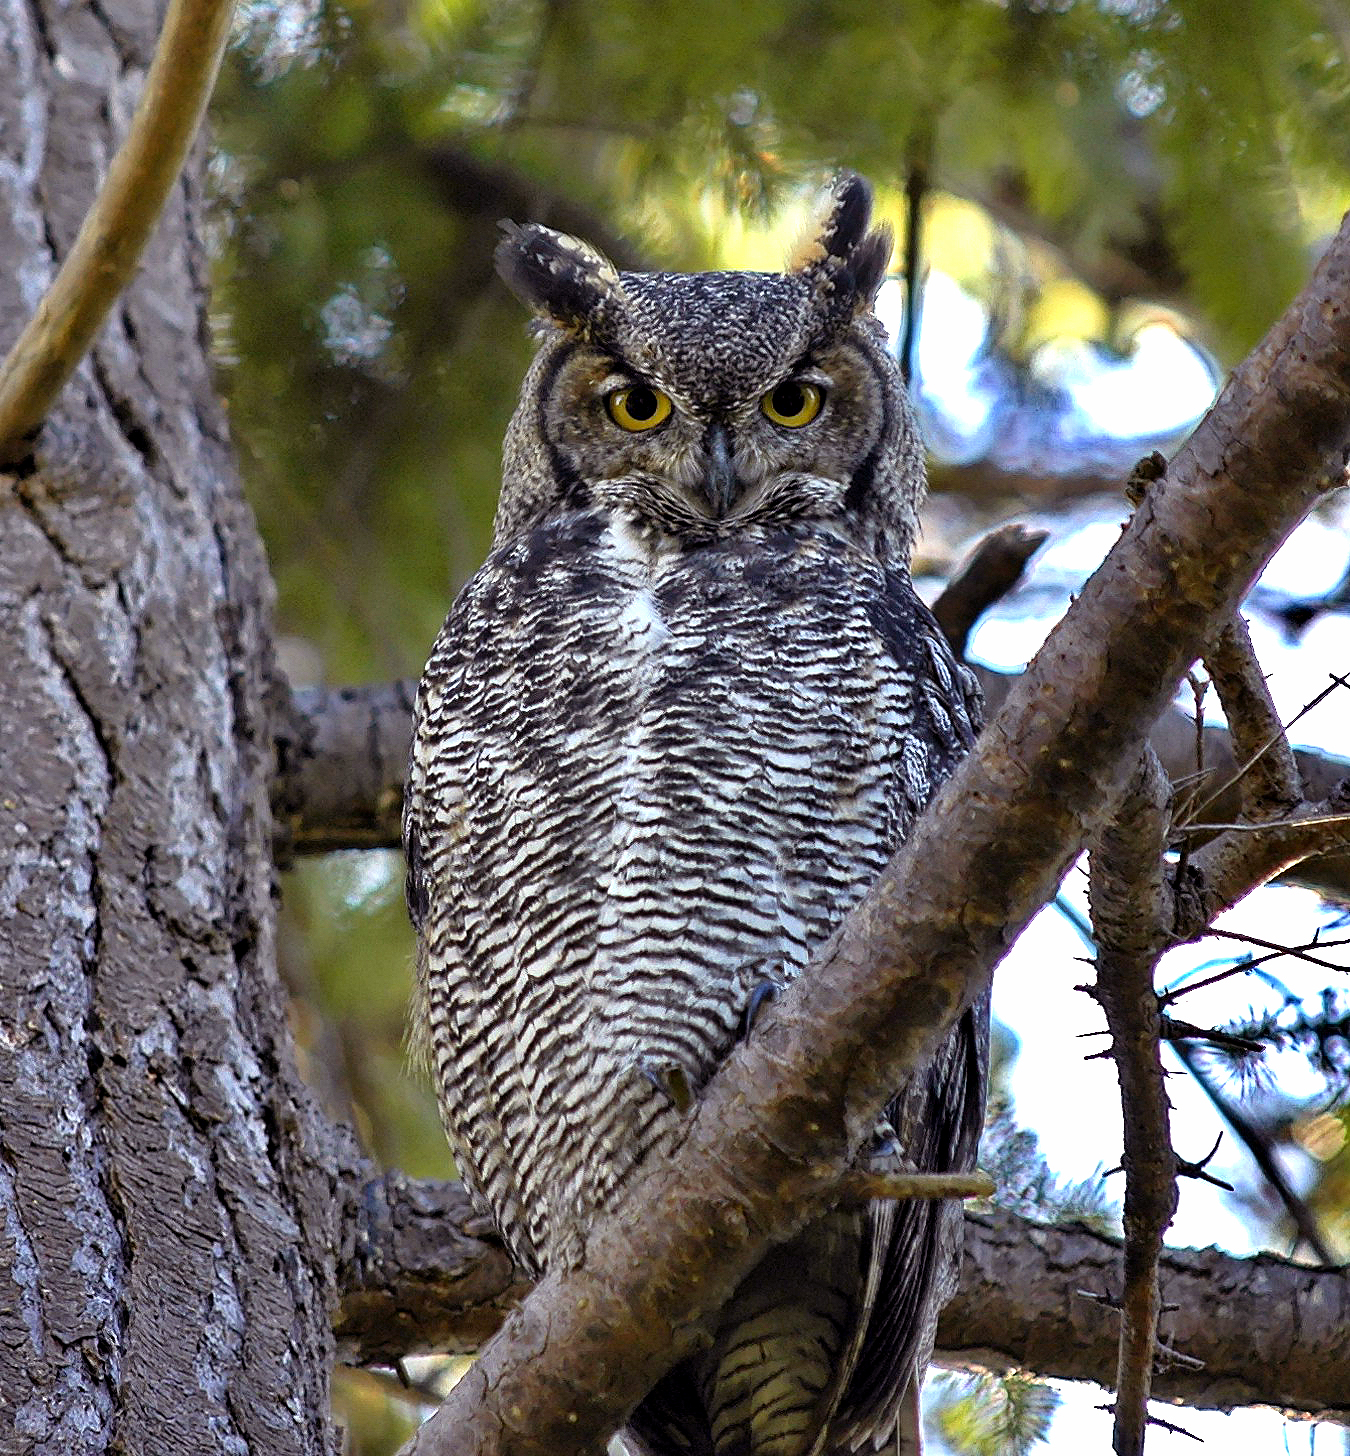
\includegraphics[width=0.8\textwidth]{owl.jpg}
		
		\EC
		
		\ECC
	}
		
		\frame{\frametitle{\bf Seeing small things}
			
			\BC \Large
			
			Surprise: a larger aperture also lets you see {\it smaller} things.
			
			\EC
			
			\normalsize
			\BI
			\item Light spreads out as it goes through a hole or past an edge
			\item This is called {\color{red} diffraction}
			\item The larger the hole, the less diffraction you get
			\EI
		\BC
		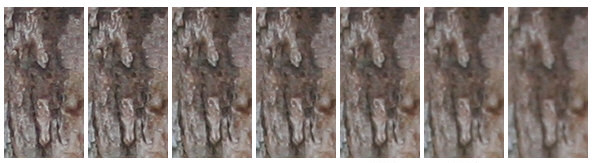
\includegraphics[width=0.95\textwidth]{bob-atkins-diffraction.jpg}	
		
		\BS
		
		\small Examples of diffraction from Bob Atkins from a camera. Left: 75 mm aperture. Right: 9 mm aperture
		\EC
		
		
		}
	
			
	\frame{\frametitle{\bf Seeing small things}
		
		\BC \large
		
			From physics, assuming perfect optics:
			
			$$ \color{white} \text{smallest detail visible} = 2.5 \times \frac{\color{yellow}\text{wavelength of light}}{\color{orange}\text{diameter of telescope}} \times {\color{green}\text{distance to object}}$$
			
{			\color{A} Assuming your optics and sensor are good, the {\it only} thing that affects \\ how much fine detail you can see is the {\bf size of the aperture.}}

\pause
			
			\BS\BS\BS
			
			Example for one of Galileo's telescopes, considering Jupiter:
			
	
$$ \color{white} \text{smallest detail visible} = 2.5 \times \frac{\color{yellow}\text{600 nm}}{\color{orange}\text{26 mm}} \times {\color{green}\text{750 million km}} \approx 50,000\,\rm{km}$$
		
			
			\BS\BS
			
			(Io is 500,000 km from Jupiter, so this would be visible!)
		
			\EC
			
}
	
		\frame{\frametitle{\bf The pursuit of bigger apertures}
				\BCC
			\column{0.7\textwidth}
			Telescopes made with lenses (like our eyeballs) have some problems:
			
		
			\BI
			\item They have to be very long (or sacrifice optical quality)
			\item Large-diameter lenses get thick, expensive, and heavy
			
			\BS\BS\BS
			
			\item They still suffer from {\it chromatic aberration}
			\BI
			\item Lenses don't focus all colors of light the same
			\item This gets worse with increasing aperture
			\item It can be partially corrected but the lenses get even bigger
			\EI
			\EI
			\column{0.3\textwidth}
			\BC
			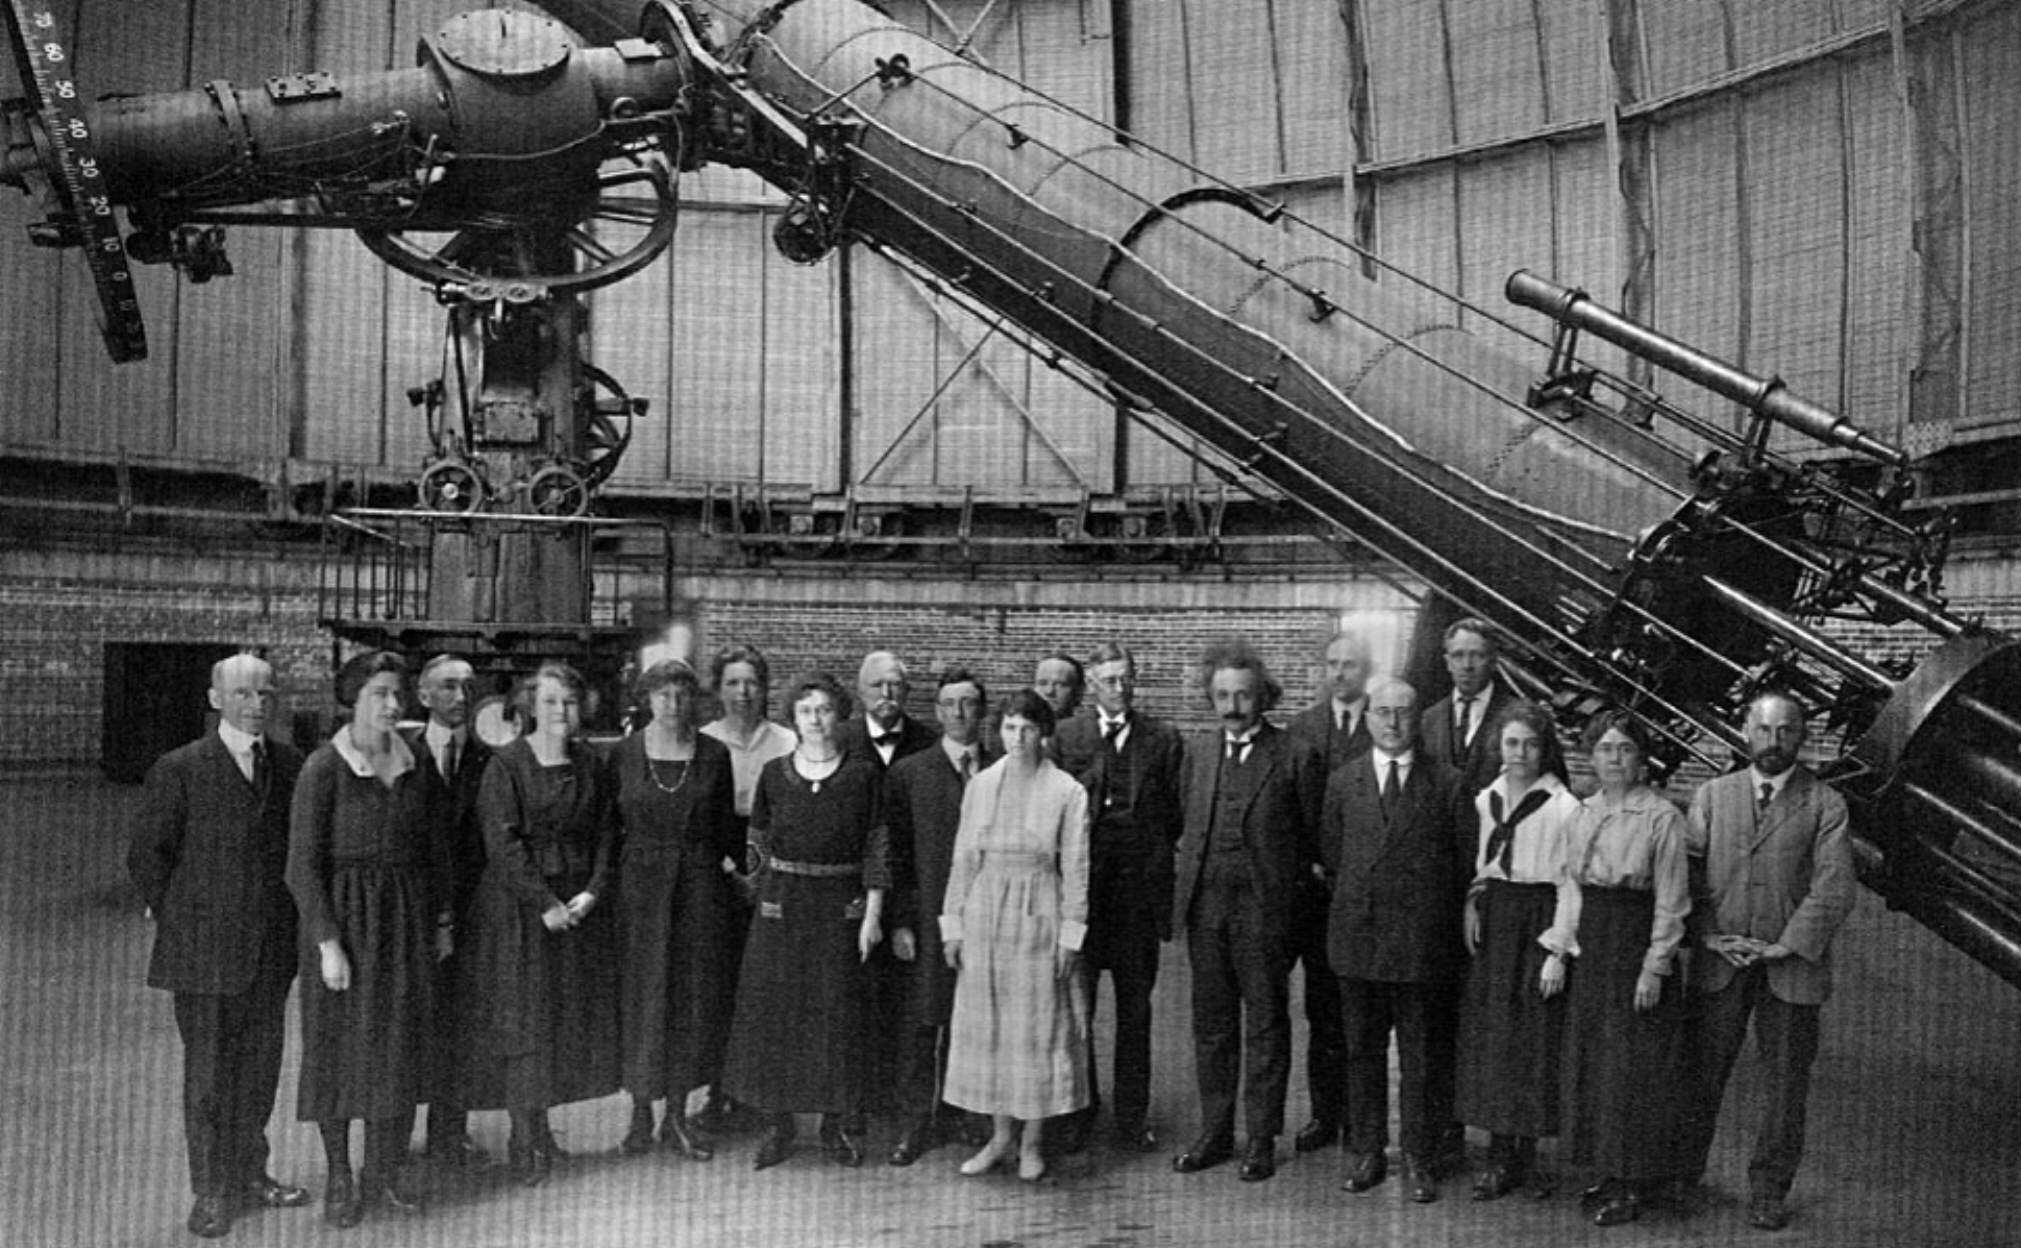
\includegraphics[width=0.9\textwidth]{big-refractor.jpg}\\
			\scriptsize 40" refracting telescope at Yerkes Observatory, 1921
			\BS\BS
						
			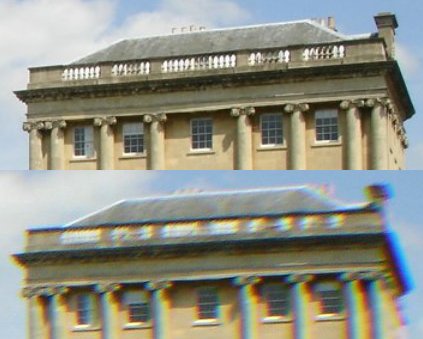
\includegraphics[width=0.9\textwidth]{chromatic-aberration.jpg}
			\\
			\scriptsize Stan Zurek / Wikimedia Commons
			\EC
			\ECC
		}
			
			
				\frame{\frametitle{\bf Solution: use mirrors}
					
					\BC
					\Large
					
					A mirror requires only a thin surface of optical material, avoids chromatic aberration, and is far easier to make.
					\BS
					
					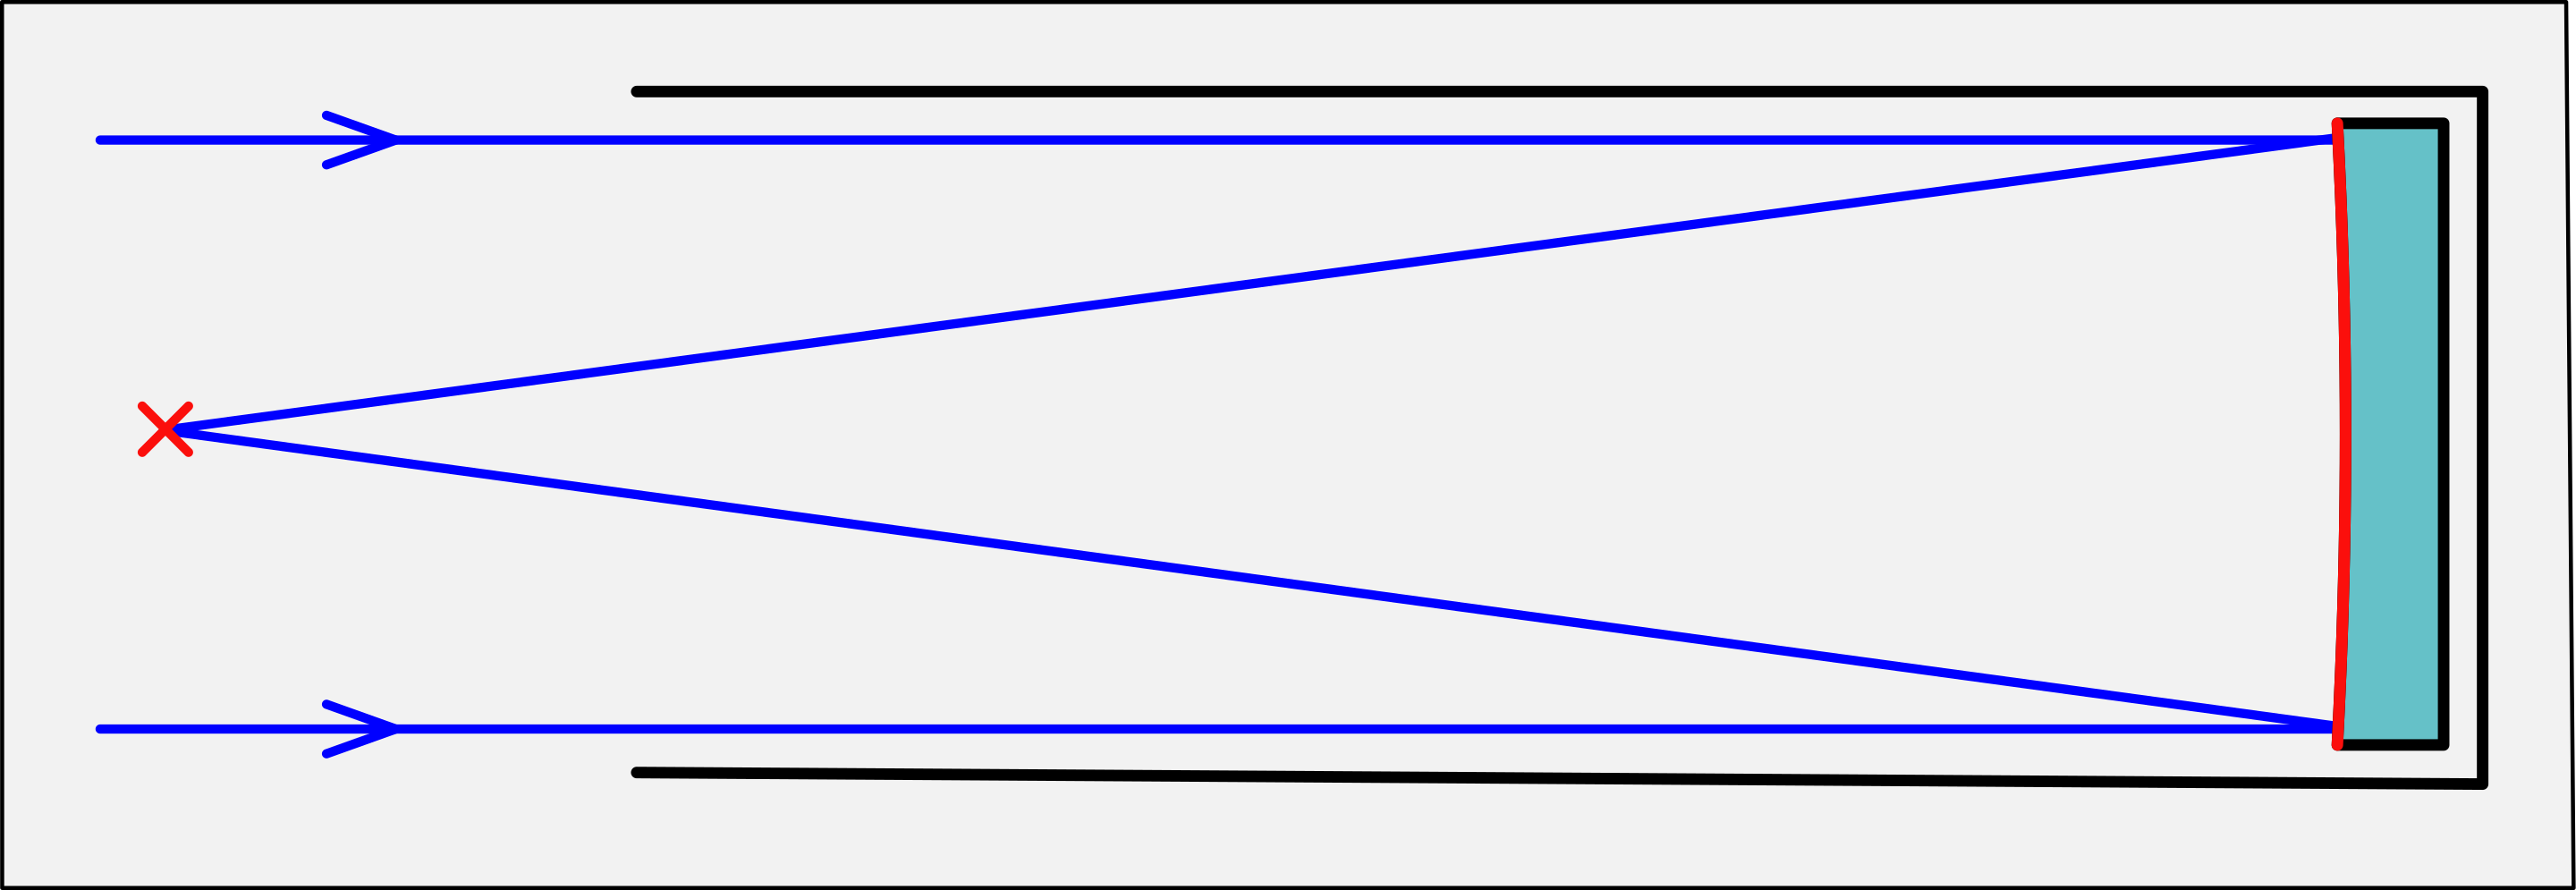
\includegraphics[width=0.6\textwidth]{prime-focus.png}\\
										\scriptsize Oleg Alexandrov / Wikimedia Commons
					
					\pause\BS\BS\BS
					
					\large
					
					{\footnotesize (Camera ``lenses'' can be made out of mirrors too!)}
					
					
								\EC		
			}
		
		\frame{\frametitle{\bf The telescope I have here is bigger than the Holden one!}
			\BCC
			\HC
			\BC
			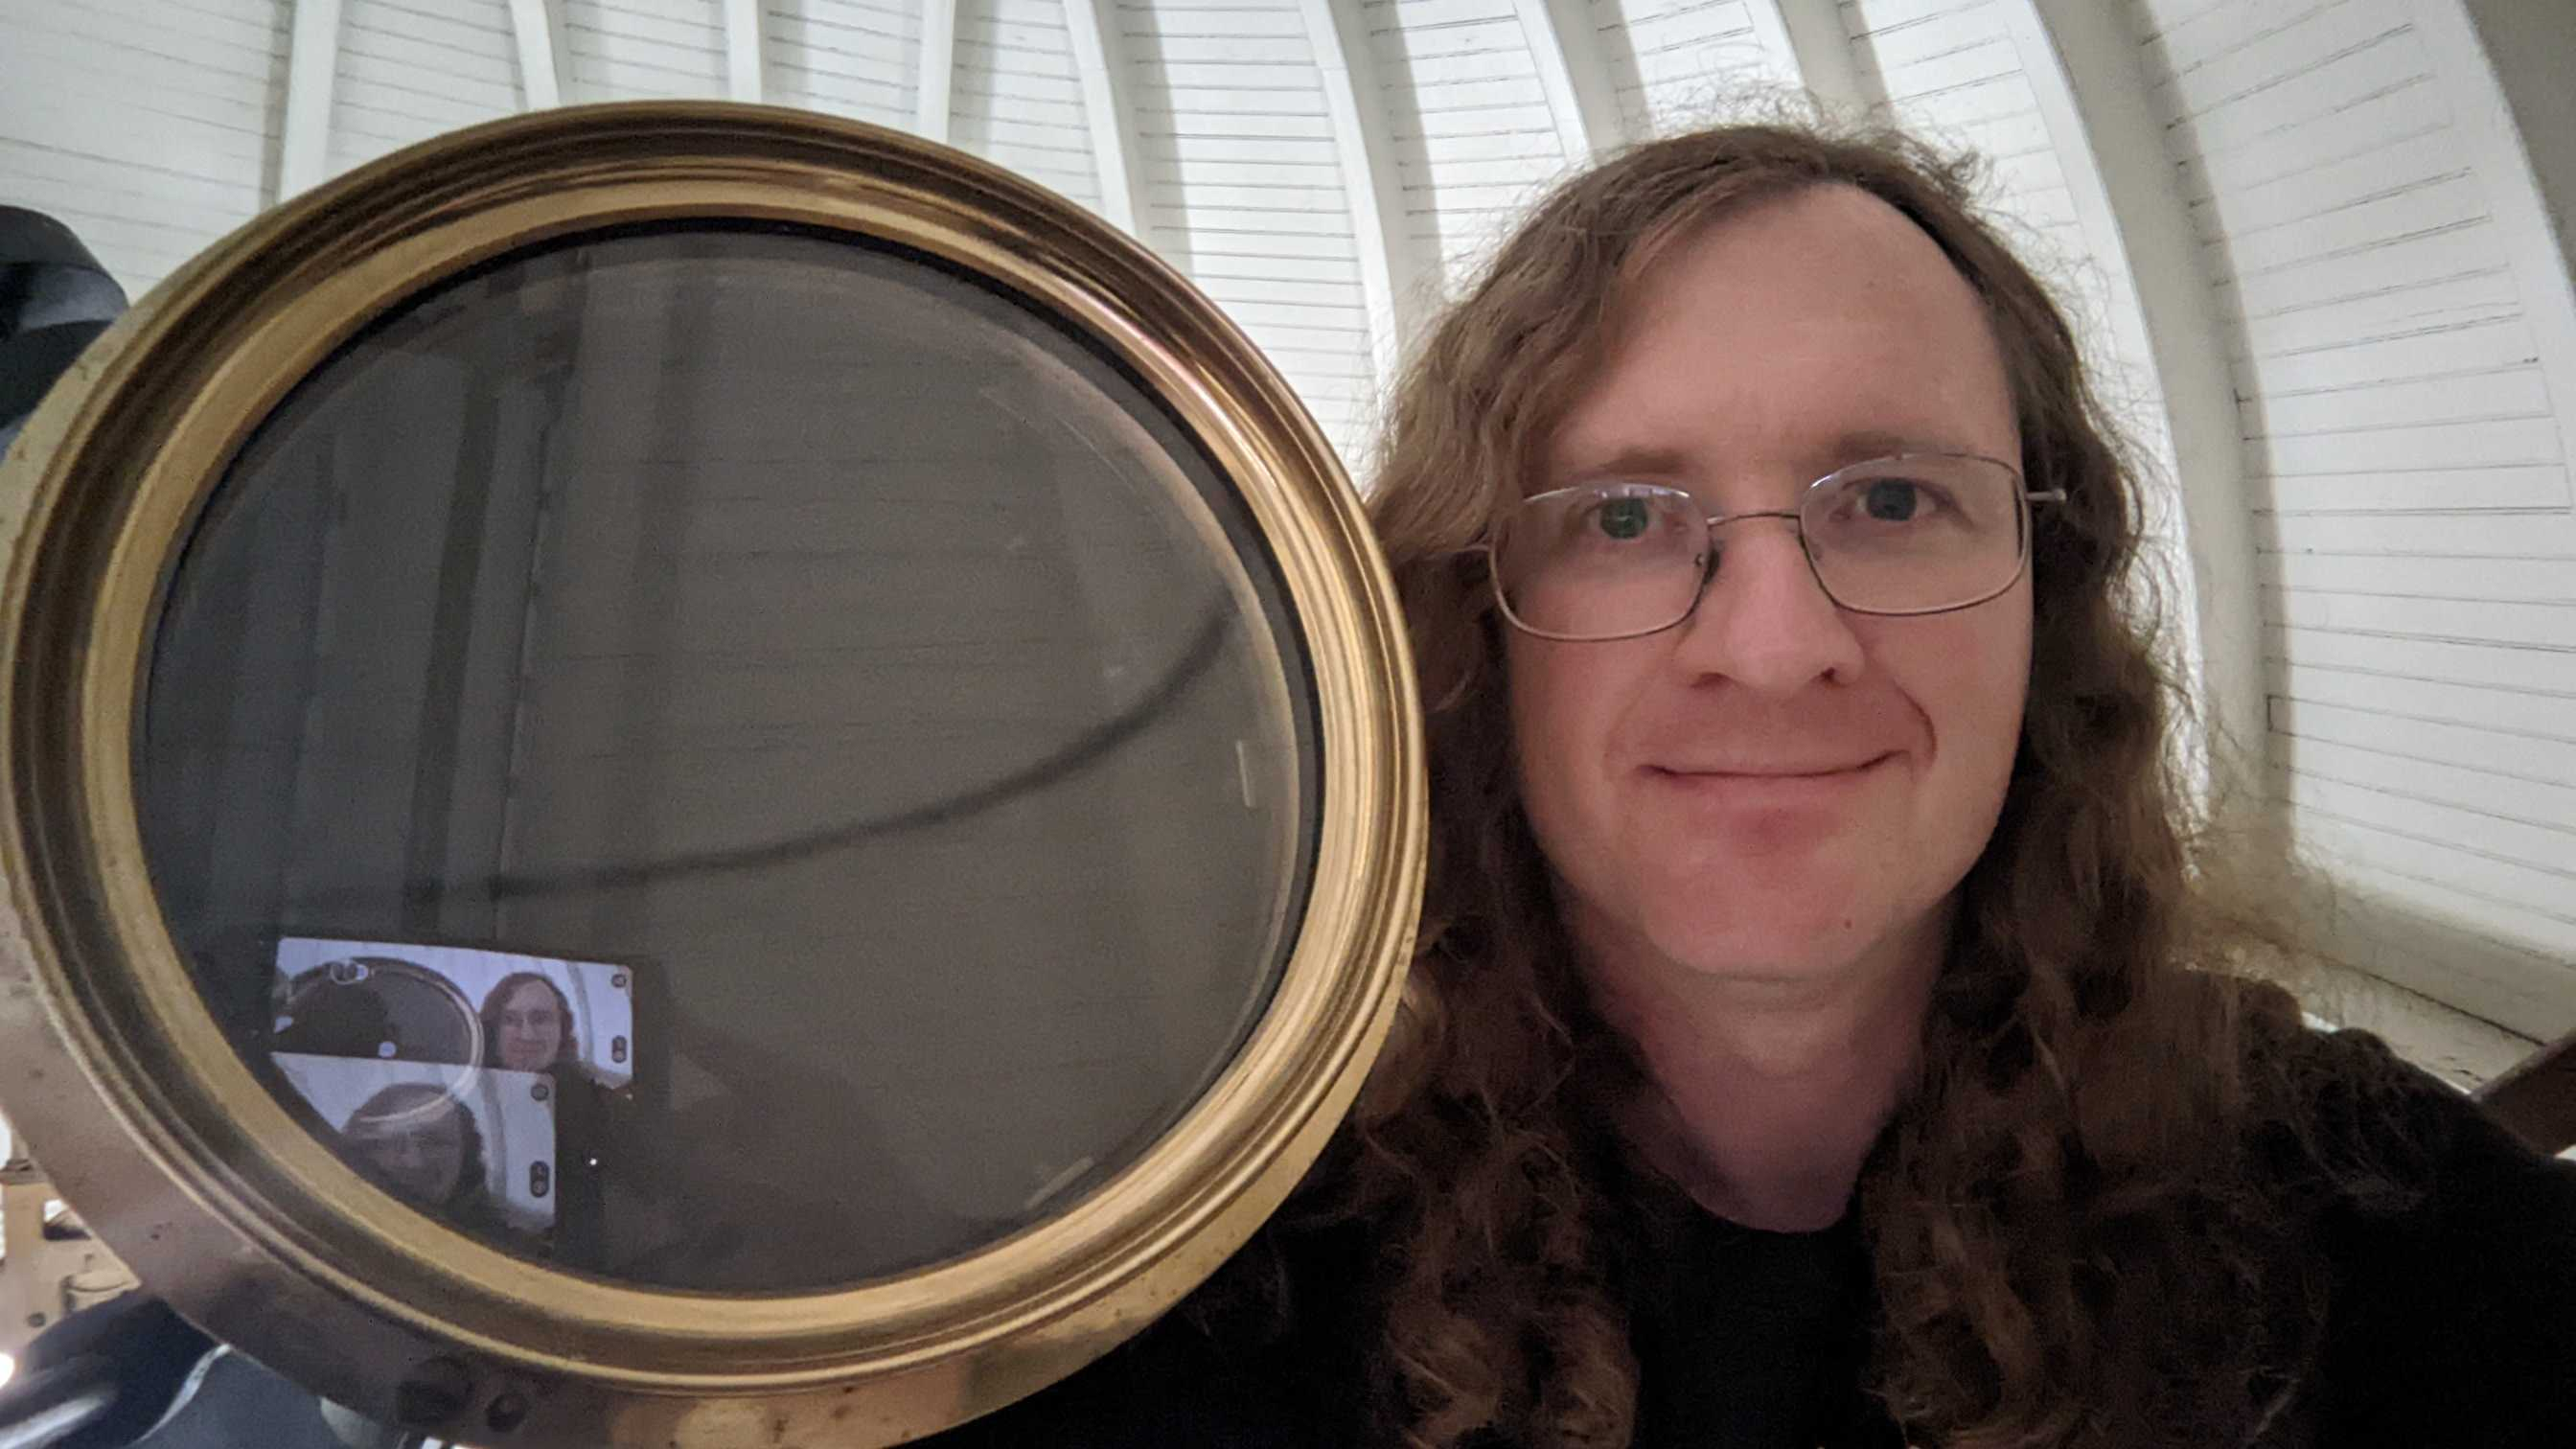
\includegraphics[width=0.9\textwidth]{selfie.jpg}
		\EC\HC
			\BC
		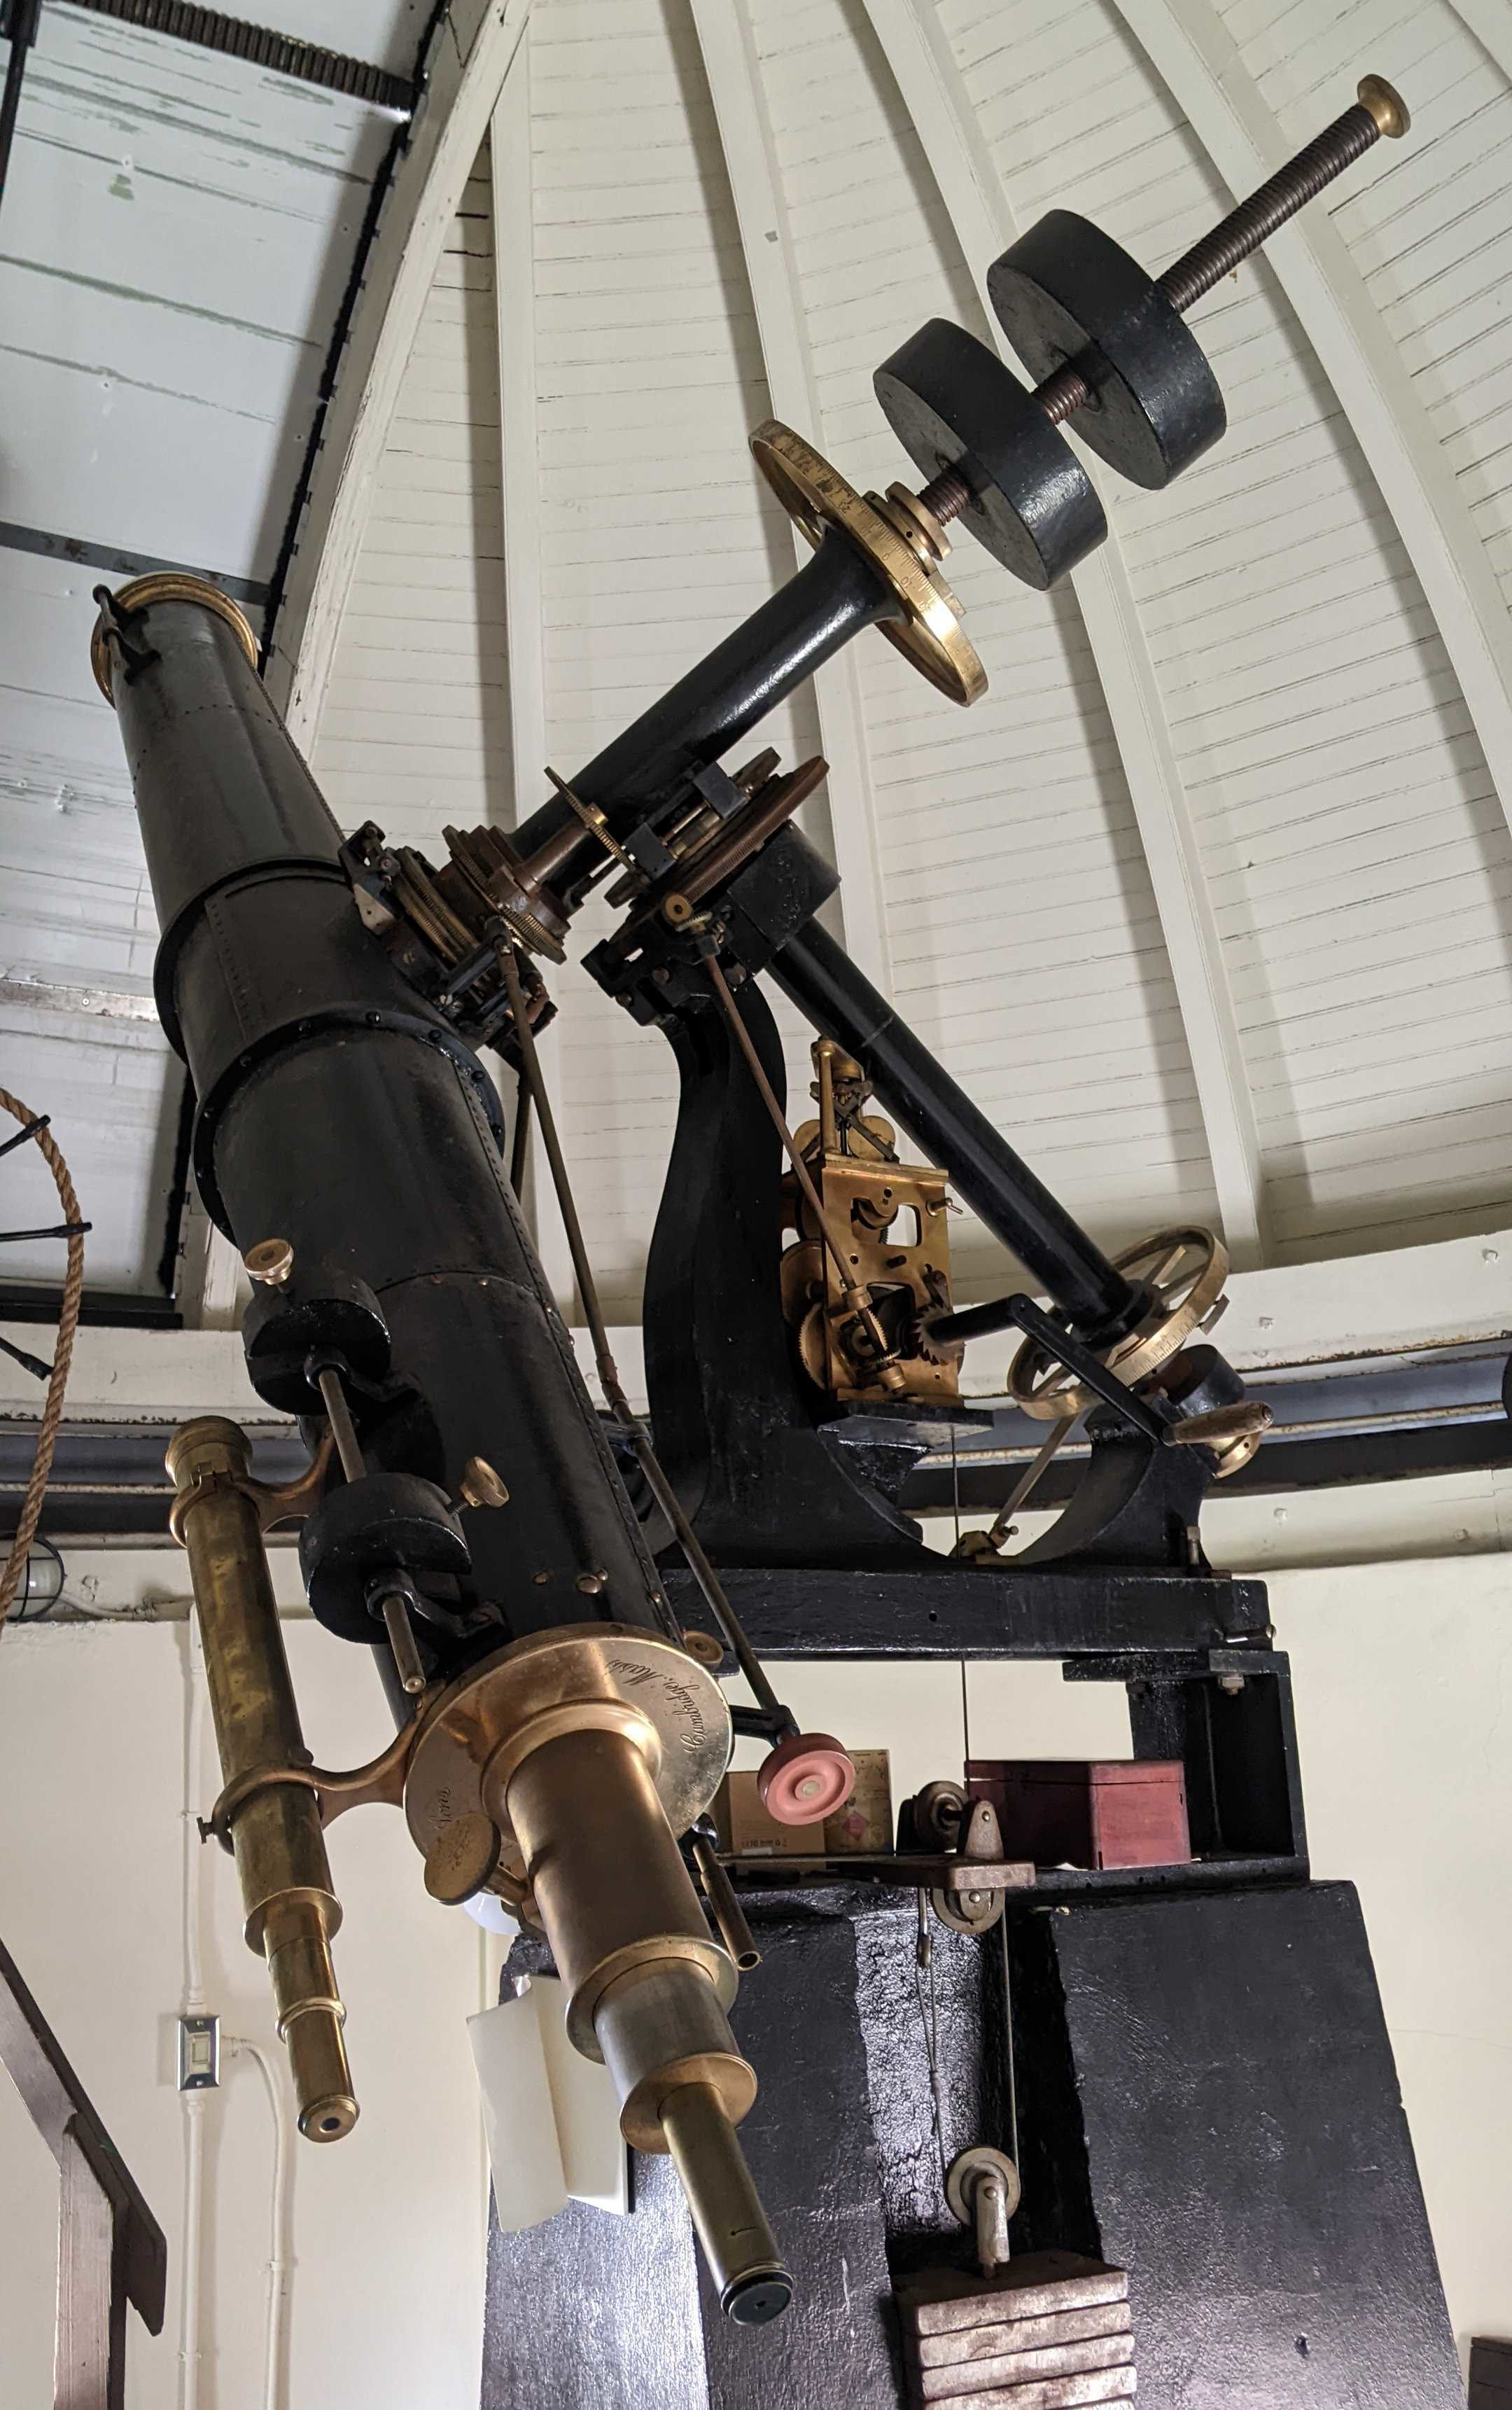
\includegraphics[width=0.7\textwidth]{holden.jpg}
		\EC
		\ECC
		
	}


		\frame{\frametitle{\bf Stop twinkling, little star!}
		
		\large
		\BC
		Stars twinkle because of random refraction from Earth's atmosphere.
		
		\BS
		
		This is pretty, but it makes astronomers grumpy.
		
		\BS\BS\pause
		
		Solution: look for dry, thin, stable air on the tops of mountains!
		
		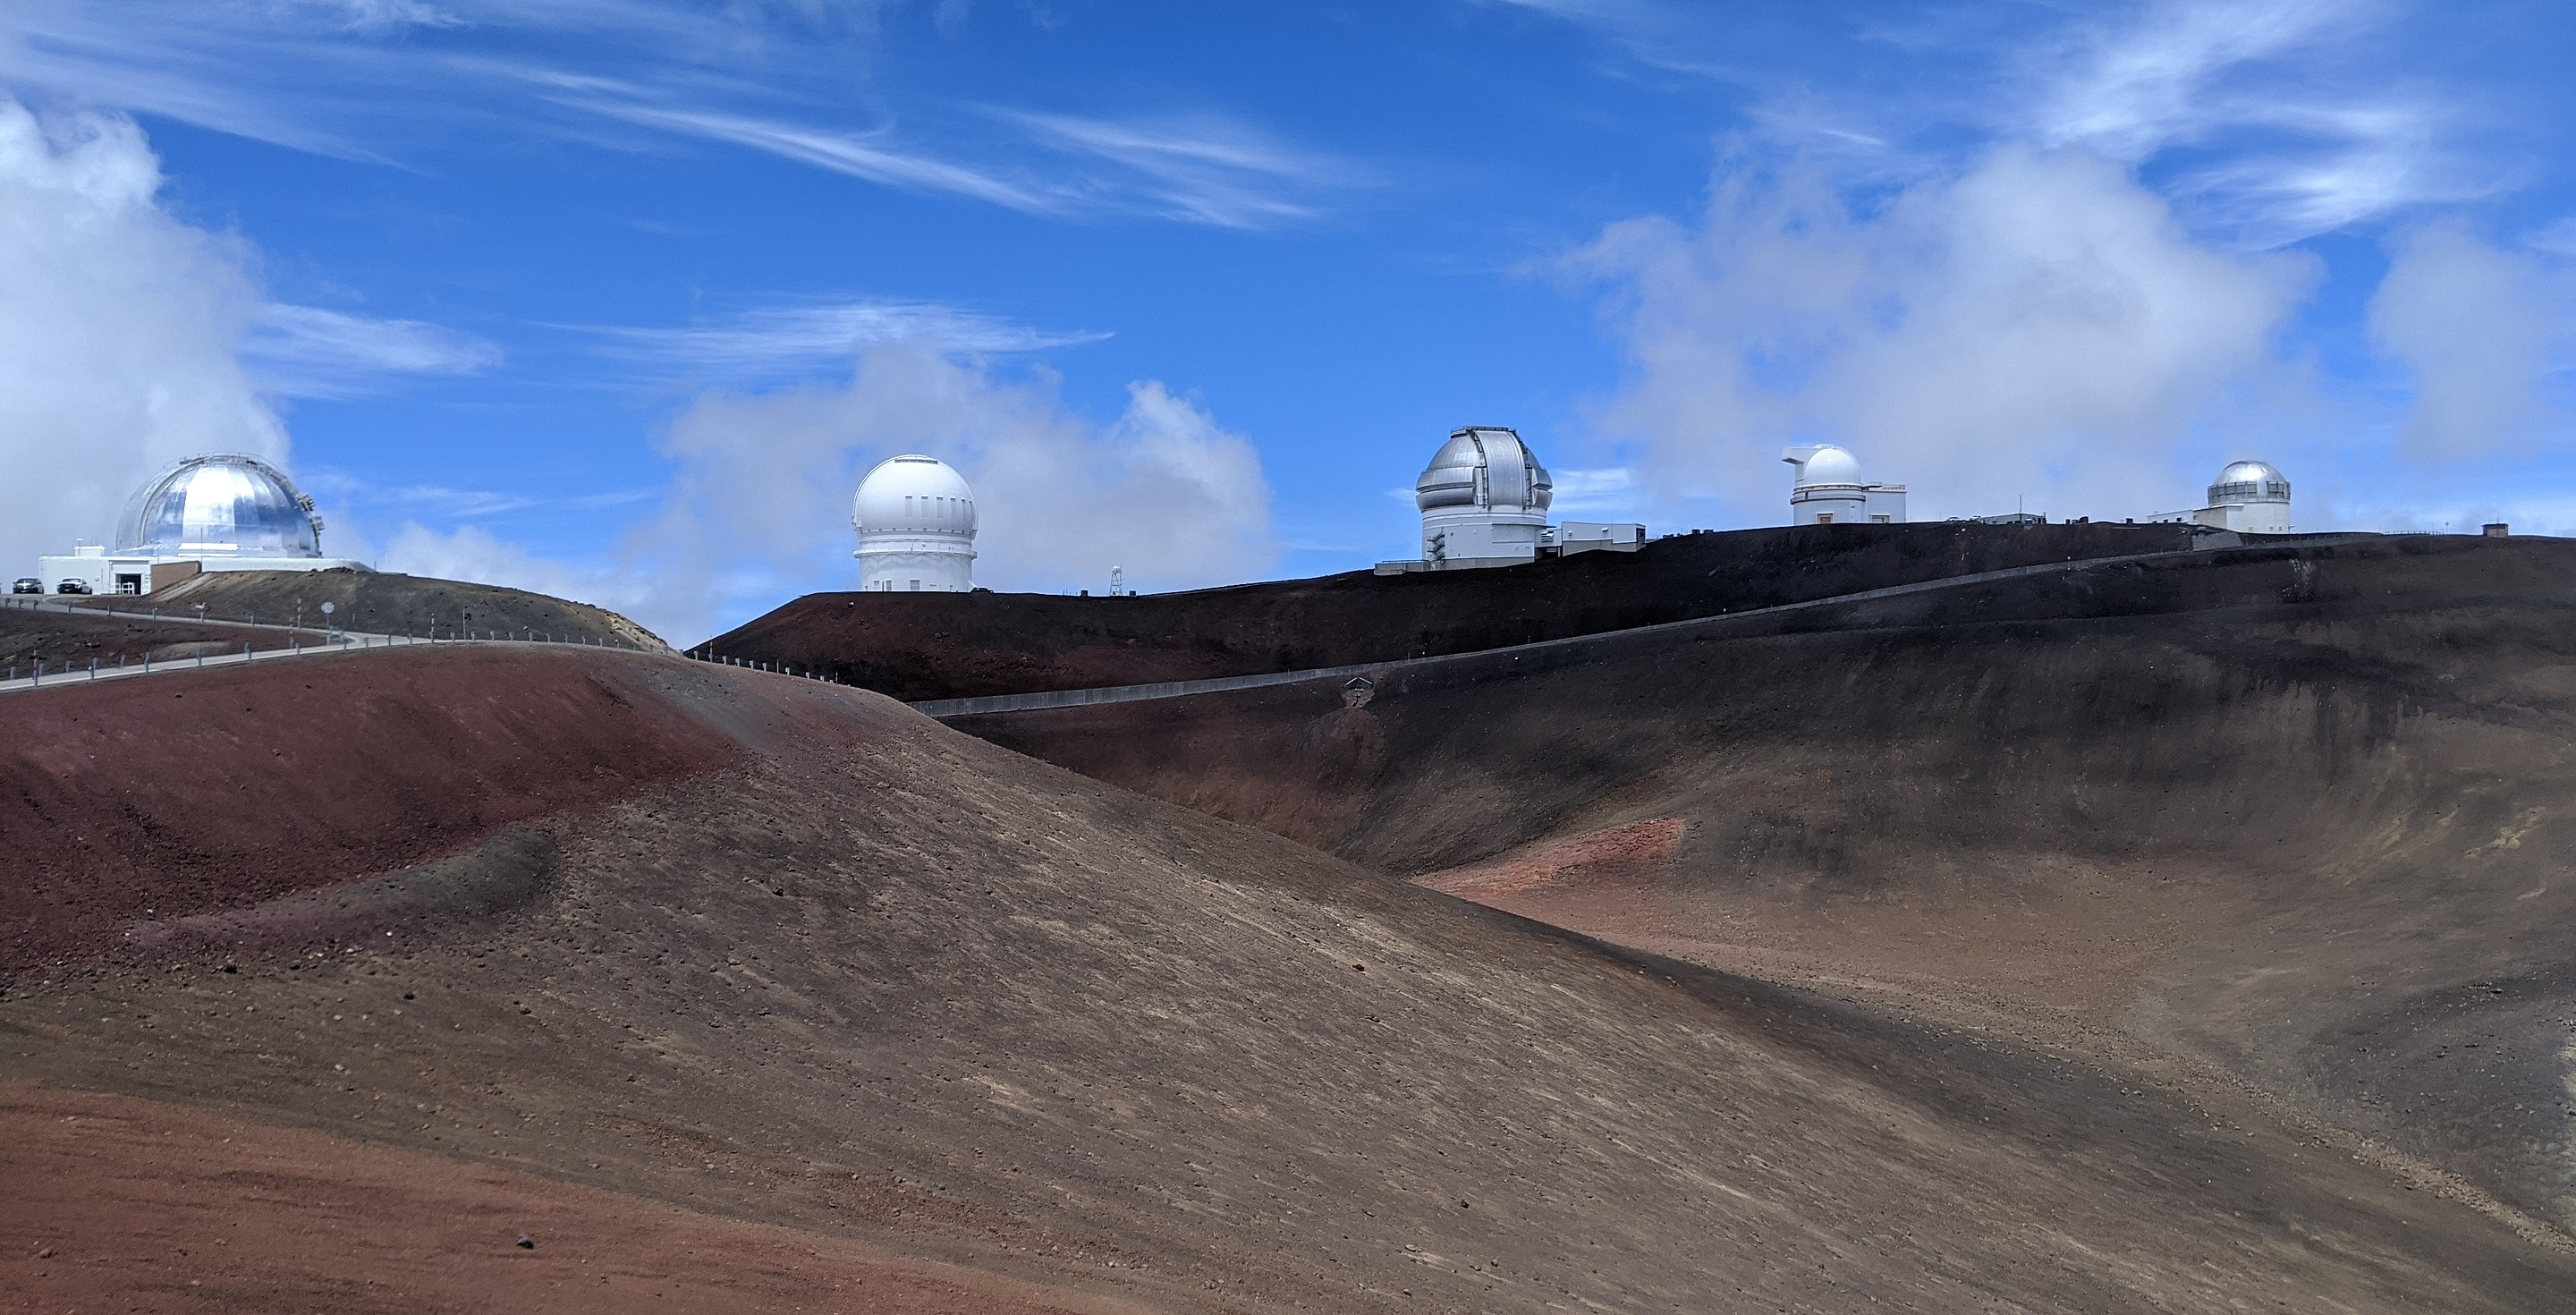
\includegraphics[width=0.7\textwidth]{mauna-kea.jpg}
		\\  \scriptsize Telescopes in Mauna Kea, Hawai'i (13,800' elevation) - Leijurv / Wikimedia Commons
		\EC
		
		}
	
	\frame{\frametitle{\bf Improving on the Holden scope, so far}
		
		\Large
		
		Now we know how to:
		
		\normalsize
		
		\BI
		\item Achieve bigger apertures with smaller telescopes using mirrors
	\BS
		
		\item Dispense with eyepieces by using film (or digital sensors) at the focal plane
	\BS
	
		\item Build telescopes in places with less twinkly skies
		\EI
\BS\BS
... what's next?

\pause

\BS

\BC
\large
Next step: improve the color ``vision'' of telescopes beyond the human eye!
\EC
}
	



\frame{\frametitle{\bf Seeing more precise color}

	\BC
\large As you know, even within the visible range, our eyes are extremely limited:
\EC
\BCC

\HC

\BC
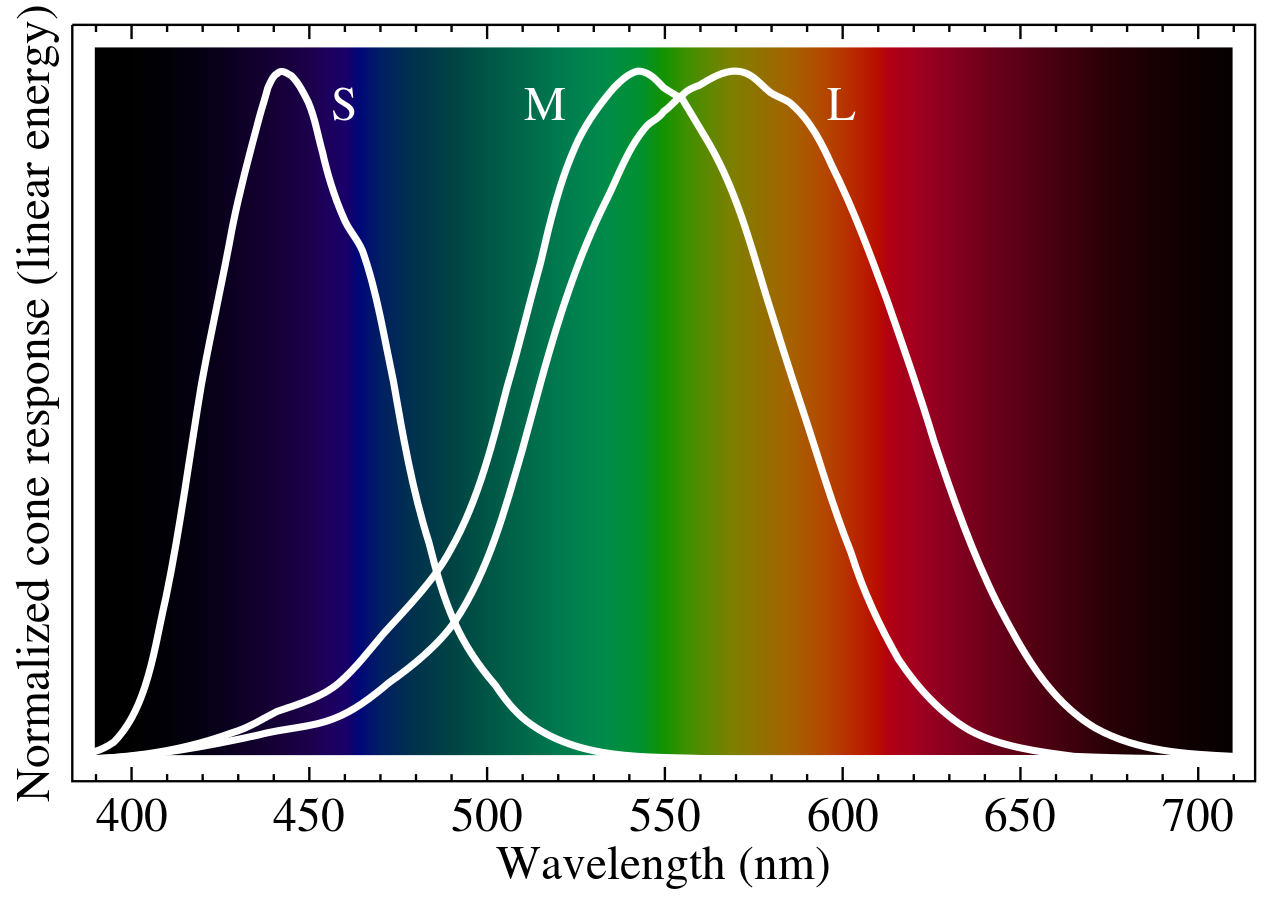
\includegraphics[width=0.9\textwidth]{cones.png}

\BS\BS

The human eye can only see three different colors.

Other shades like orange are a mixture of these.
\EC

\HC
\BC
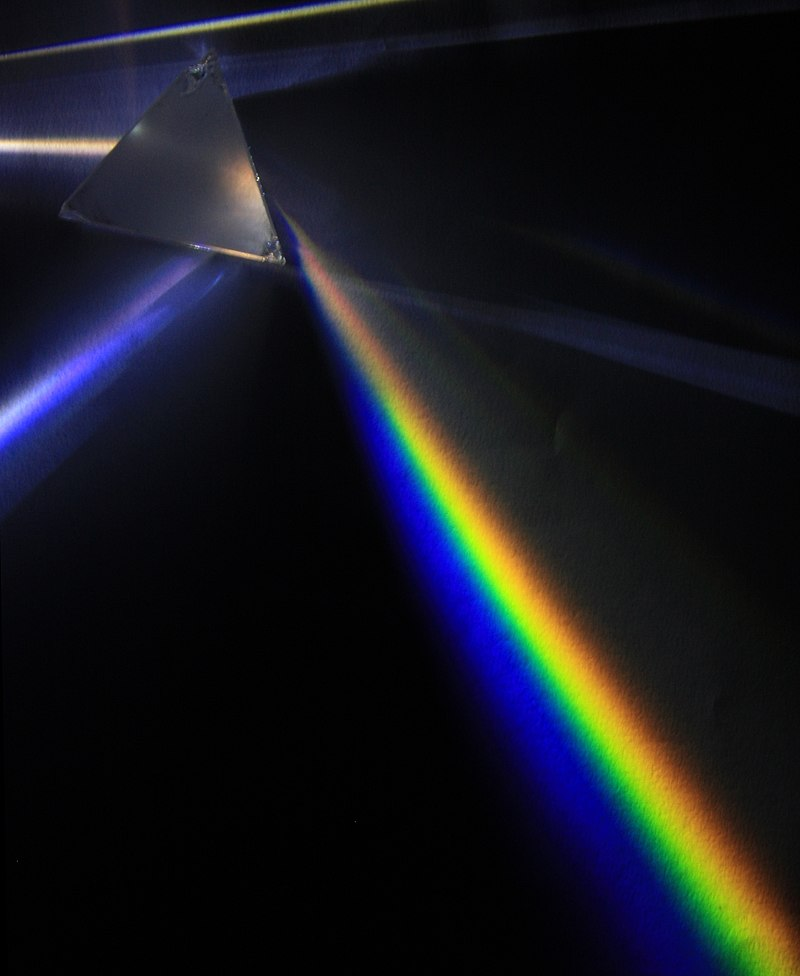
\includegraphics[width=0.5\textwidth]{prism.jpg}

\vspace{3em}

Solution: separate out the wavelengths of light
using a prism (then) or diffraction grating (now)

\EC
\ECC
}

\frame{\frametitle{\bf Seeing a wider range of colors}
	
	\begin{center}
		
		\large As you know, there is a vastly wider range of light than we can see.
		
		\BS
		
		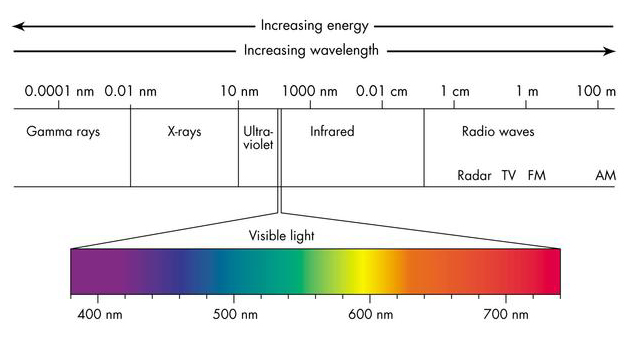
\includegraphics[width=0.5\textwidth]{em-spectrum-color.jpg}
		
		\BS\BS\pause
				
		That's okay -- we already know eyes aren't great companions to telescopes.
		
		\BS\BS
		
		\BI
		\item Photodetectors (even film) can see a much wider range of colors
		\item Colors near the visible range reflect from mirrors too!
		\EI
	\end{center}
}




		\frame{\frametitle{\bf The spectroscopic revolution}
		
		\BC
		
		There's a wealth of information about stars we can get from their spectra.
		
		\BS
		
		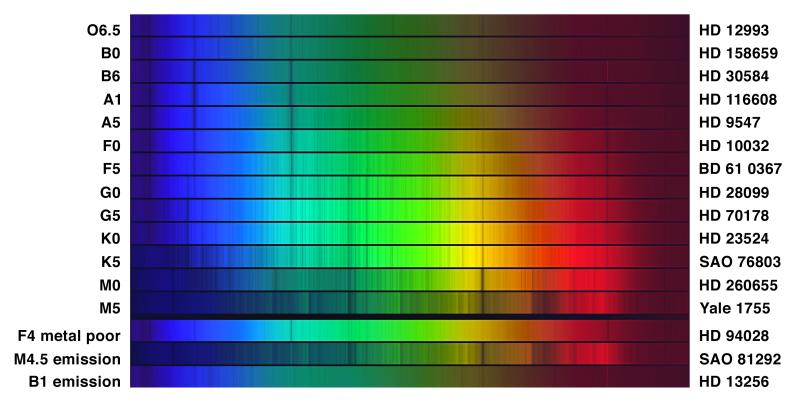
\includegraphics[width=0.8\textwidth]{stellar-spectra.jpg}

		
		\BS
		All stars mostly have the same spectral lines, but their prominence tells us things like stars' temperatures and compositions.
		\BS
		\EC		
		
	}

\frame{\frametitle{\bf The spectroscopic revolution}
	
	\BC
	
	``There are holes in the rainbow and they tell us we are made of stardust''.
	
	\BS
	
	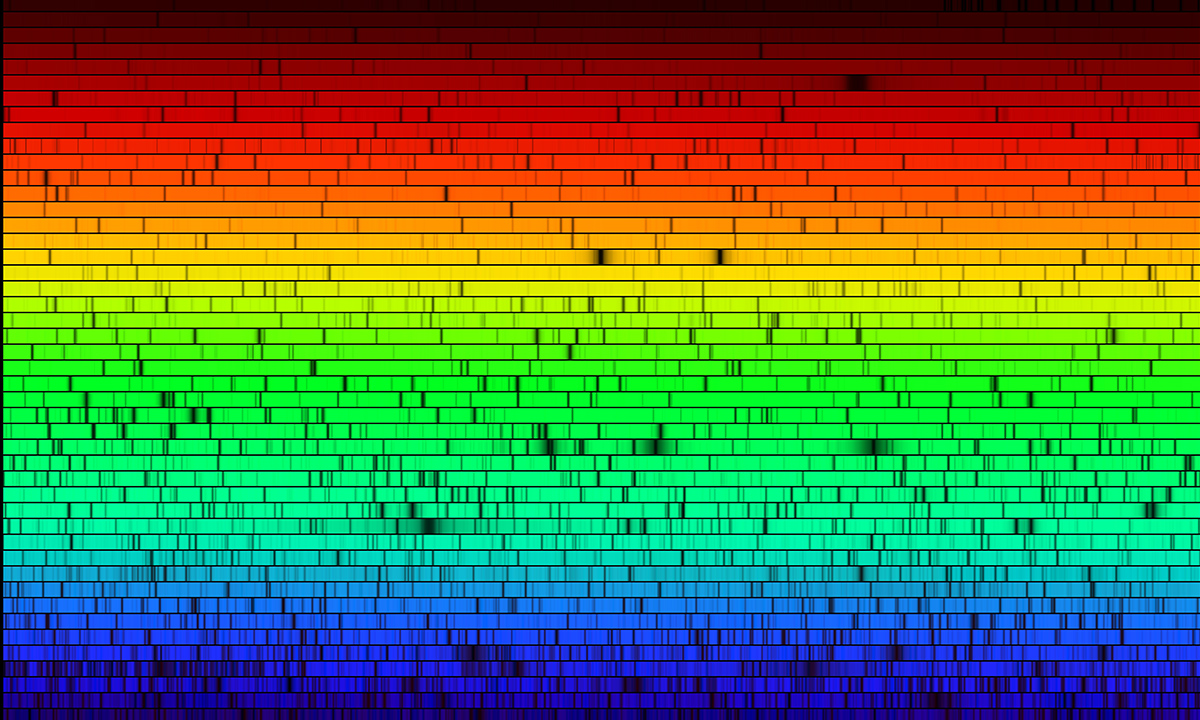
\includegraphics[width=0.8\textwidth]{solar-spectrum.jpg} \\
	\it \scriptsize (NASA / public domain)
	\EC
}

\frame{\frametitle{\bf The need for all wavelength bands}
	
	\BC
	
	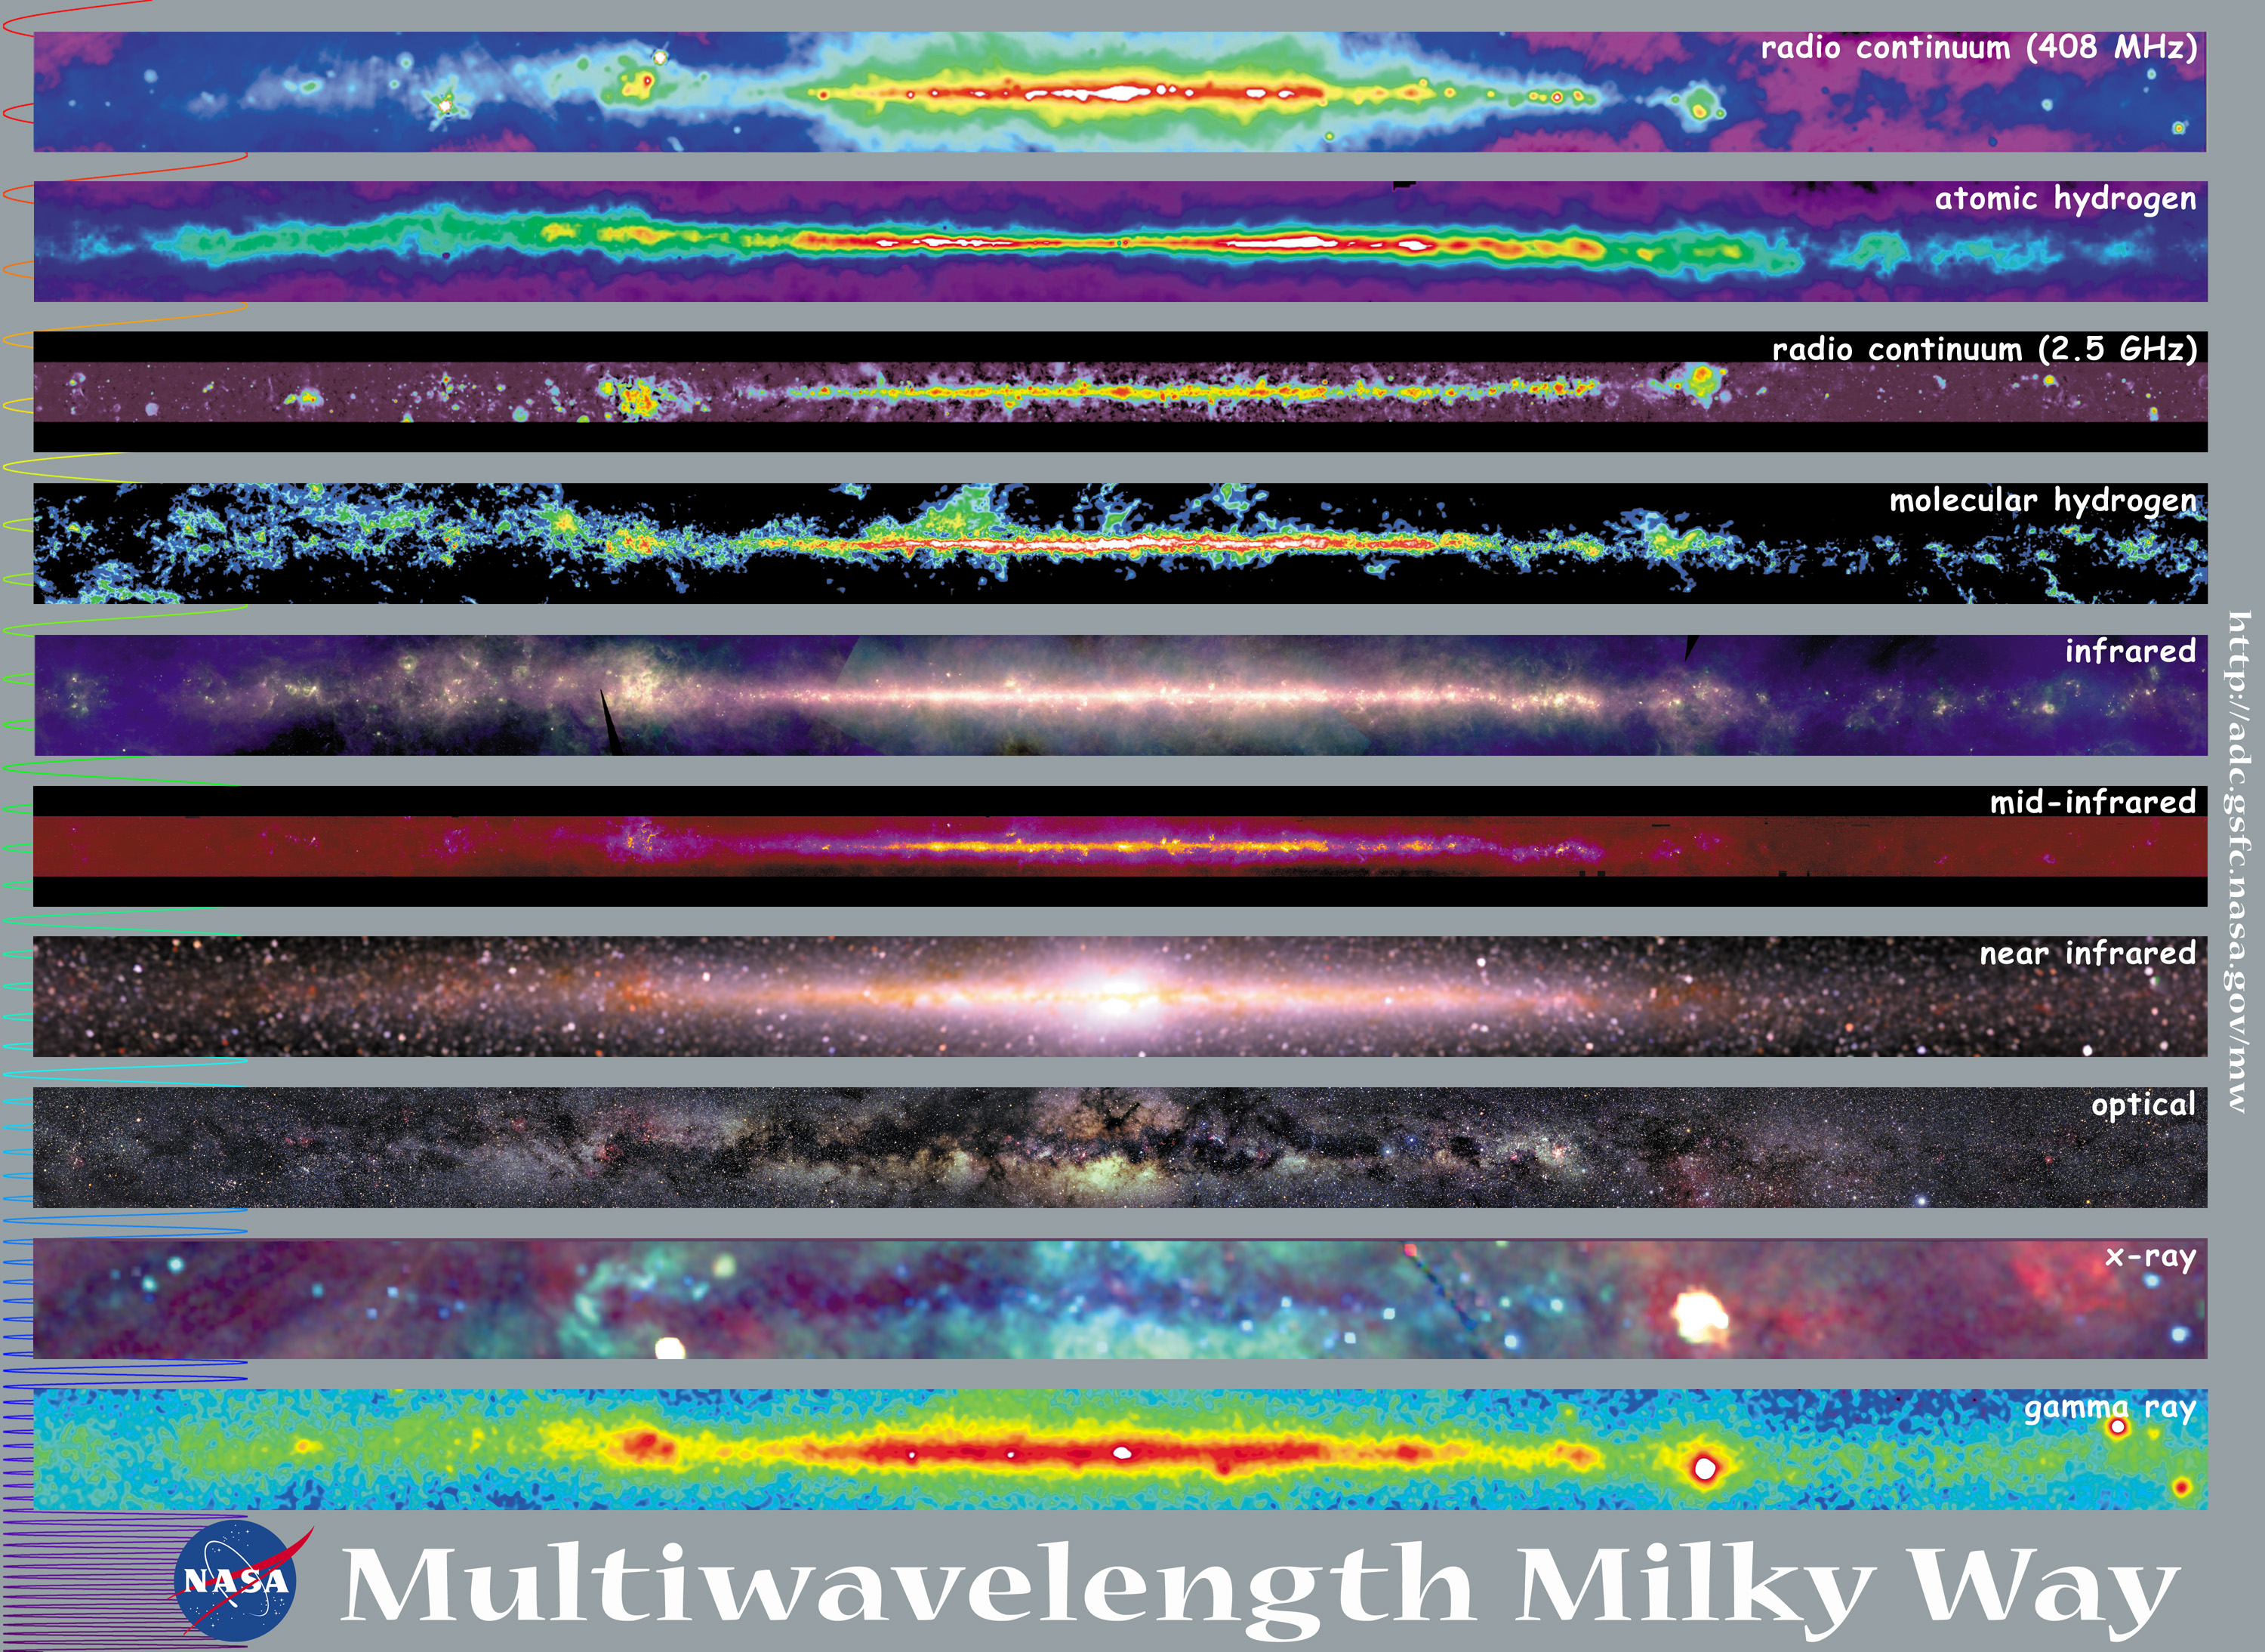
\includegraphics[width=0.8\textwidth]{mwmw.jpg}
	
	\EC
}

\frame{\frametitle{\bf The atmosphere is a problem (again)}
	
	\BC
	
	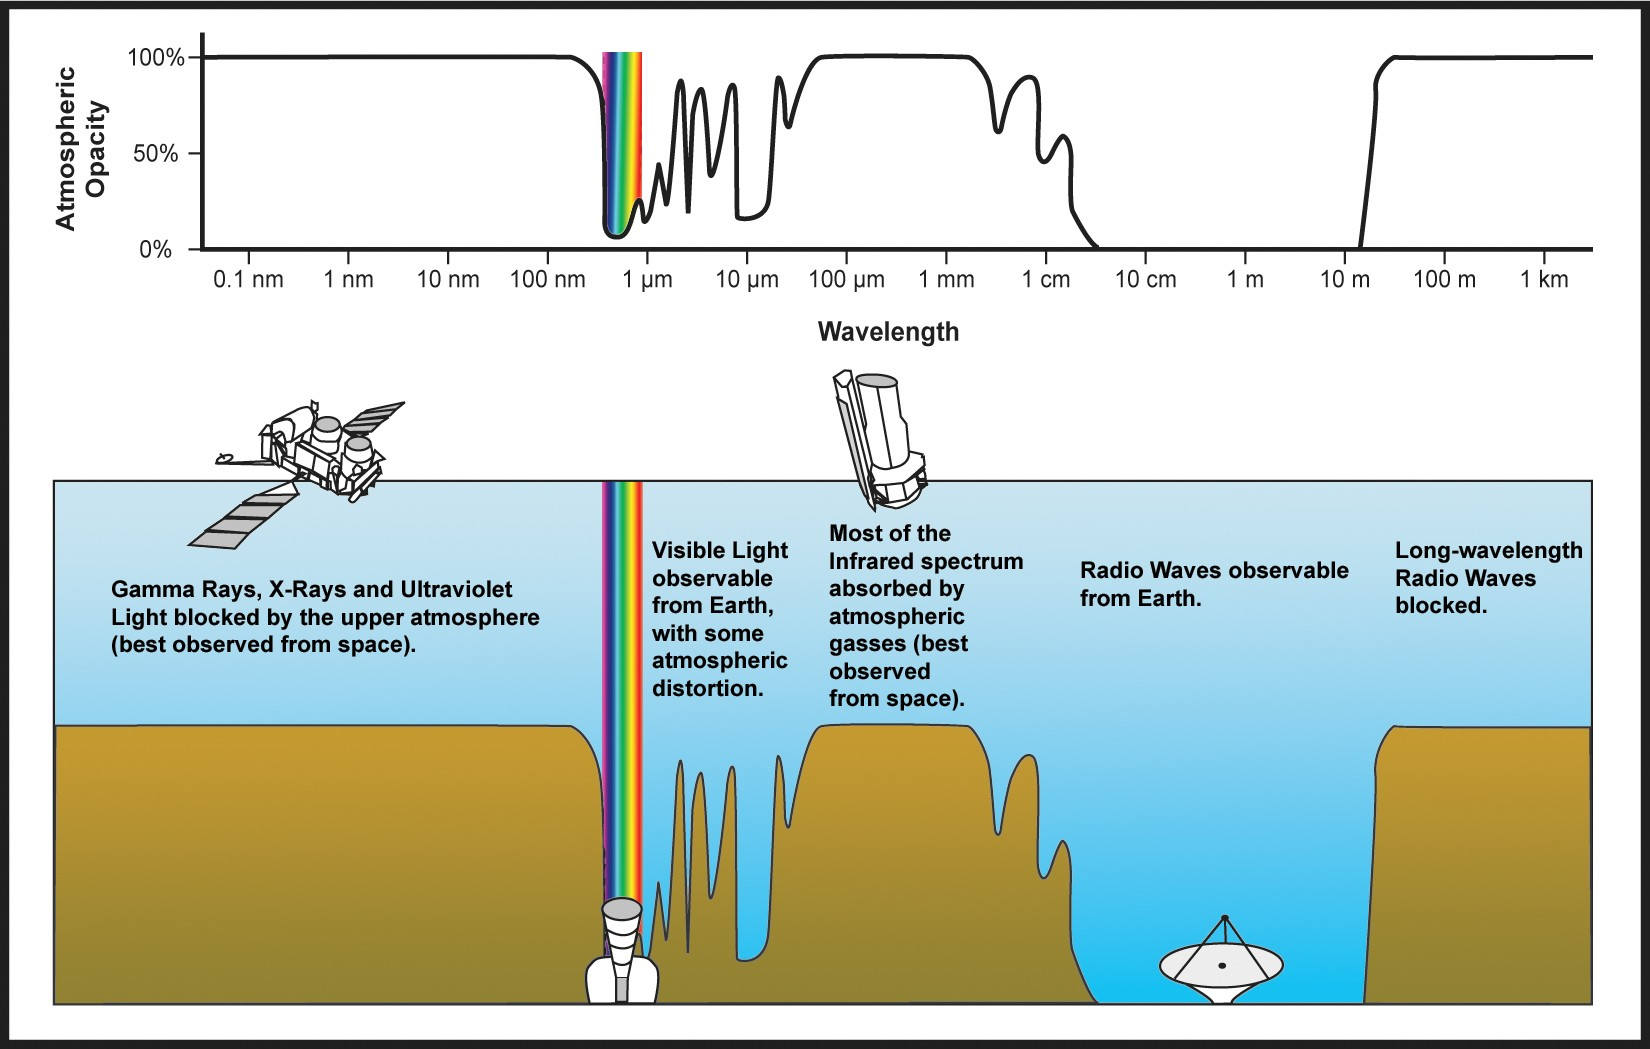
\includegraphics[width=0.8\textwidth]{atmospheric-transmittance.jpg} \\
\it \scriptsize (NASA / public domain)
	
	\BS
	
	\large Astronomy in the infrared and ultraviolet is very hard to do from Earth!
	
	\EC	
}

\frame{\frametitle{\bf Why the infrared matters, I}

\BC

\large

Planetary scientists are interested in atmospheres.


\BS

\normalsize

We can't see the signatures of chemicals in other planets' atmospheres if ours is in the way!
\BS


	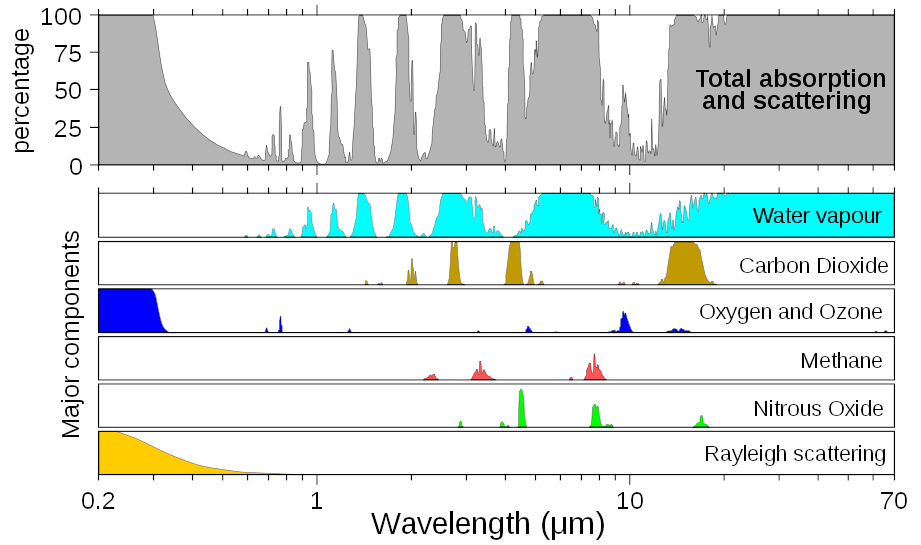
\includegraphics[width=0.75\textwidth]{atmospheric-transmission-3.png}	\\
	\scriptsize \it Wikimedia Commons / Global Warming Art Project

\EC


}


\frame{\frametitle{\bf Why the infrared matters, II: the redshift}

\Large
The Doppler effect means that light from things moving away from us \\ is shifted to longer wavelengths.

\normalsize
\BS

Since red light has longer wavelengths than blue light, this is called the ``redshift''.

\BS

\BCC
\column{0.3\textwidth}
\BC
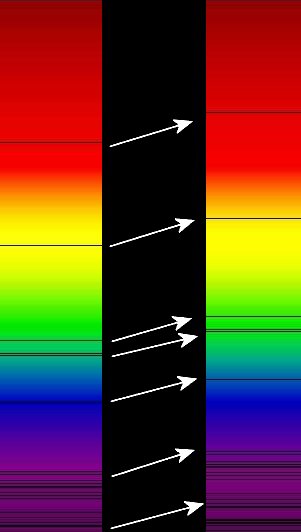
\includegraphics[width=0.7\textwidth]{redshift.png}\\
\tiny \it Georg Wiora / Wikimedia Commons
\EC
\column{0.7\textwidth}

We can figure out relative motion of stars from their Doppler shift.

\BS\BS

Surprise: 

\BI
\item Most everything is moving away from us \pause
\item The more distant they are the faster they're moving away \pause
\item {\color{A} This is a really big deal} and you will discuss it at length in AST104
\pause
\item The oldest and furthest things in the Universe are redshifted by a {\it huge} factor:
\BI
\item \color{green}Oldest galaxies: 15x wavelength
\item \color{yellow}Oldest stars: 20-30x wavelength
\EI
\EI
\ECC
}

%\frame{\frametitle{\textbf{Two sources of long-wavelength infrared light}}
%	
%	\large
%	
%	Recall:
%	
%	\BI
%	\item \color{C} An object heated to thousands of degrees (like the Sun) produces mostly light around 500-1000 nm
%	\item \color{A} An object heated to hundreds of degrees (like the Earth) produces mostly light around 5000-10000 nm
%	\EI
%
%\BS\BS\pause
%	
%	This means that {\it two kinds of sources} produce the same wavelengths of infrared light:
%	
%	\begin{itemize}
%		\item \color{C} The Earth (hundreds of degrees)
%		\item \color{A} The oldest stars (thousands of degrees, redshifted by 10x)
%	\end{itemize}
%\pause
%
%\BS\BS\BC\color{B} To see the oldest stars, we must:
%
%\BI
%\item Build an infrared telescope
%\item 
%}

\frame{\frametitle{\bf Telescopes in space: Hubble}
	
	\BC
	\Large
	Putting a telescope in space lets us see into the infrared!
	
	\normalsize (and avoid the other problems the atmosphere causes too)
	
	\BS\BS
	
	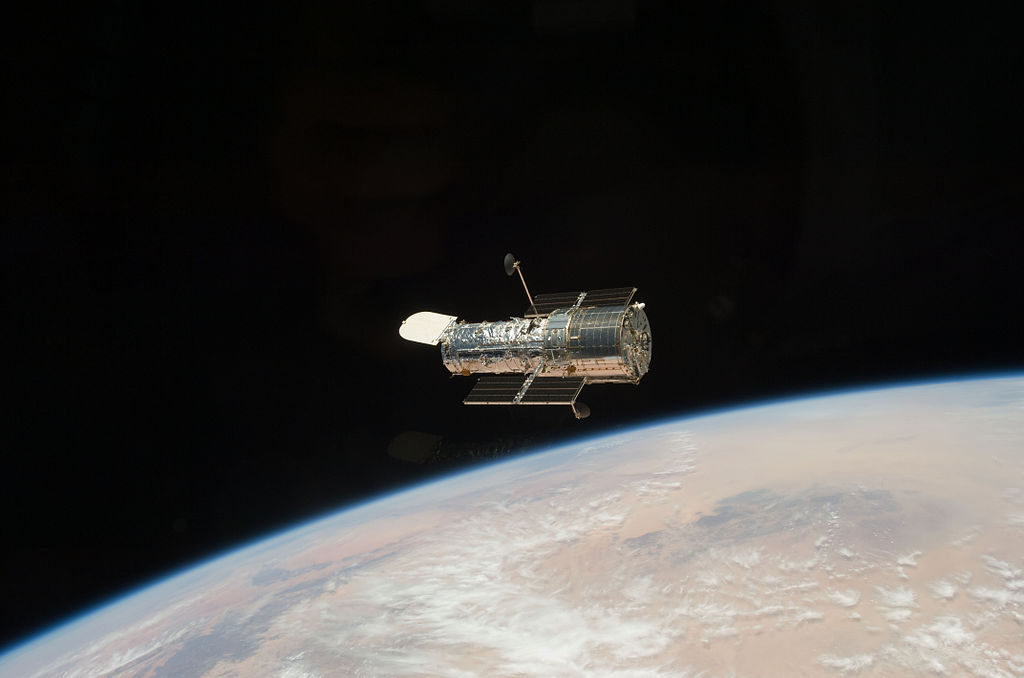
\includegraphics[width=0.7\textwidth]{hubble.jpg}
	
	\EC
}
	
\frame{\frametitle{\bf Telescopes in space: Hubble}
	
	\BC
	\Large
	Putting a telescope in space lets us see into the infrared!
	
	\normalsize (and avoid the other problems the atmosphere causes too)
	
	\BS

\BI
\item Visible + near-infrared telescope in low earth orbit
\item Sensitive from 90 - 2400 nm (ultraviolet to near infrared)
\EI

	\BS

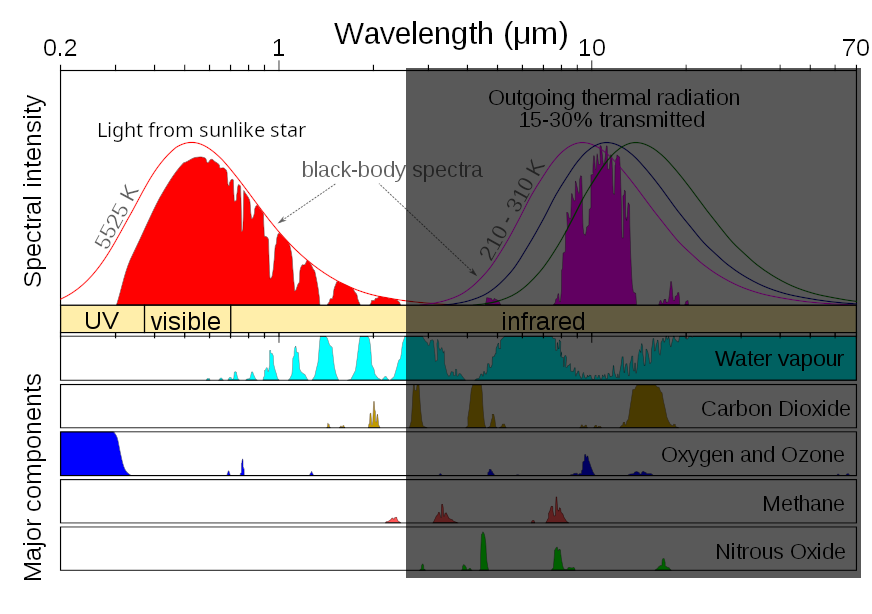
\includegraphics[width=0.55\textwidth]{hubble-sensitivity.png}

\EC

}
	
\frame{\frametitle{\bf Hubble was the new hot thing!}
\BC
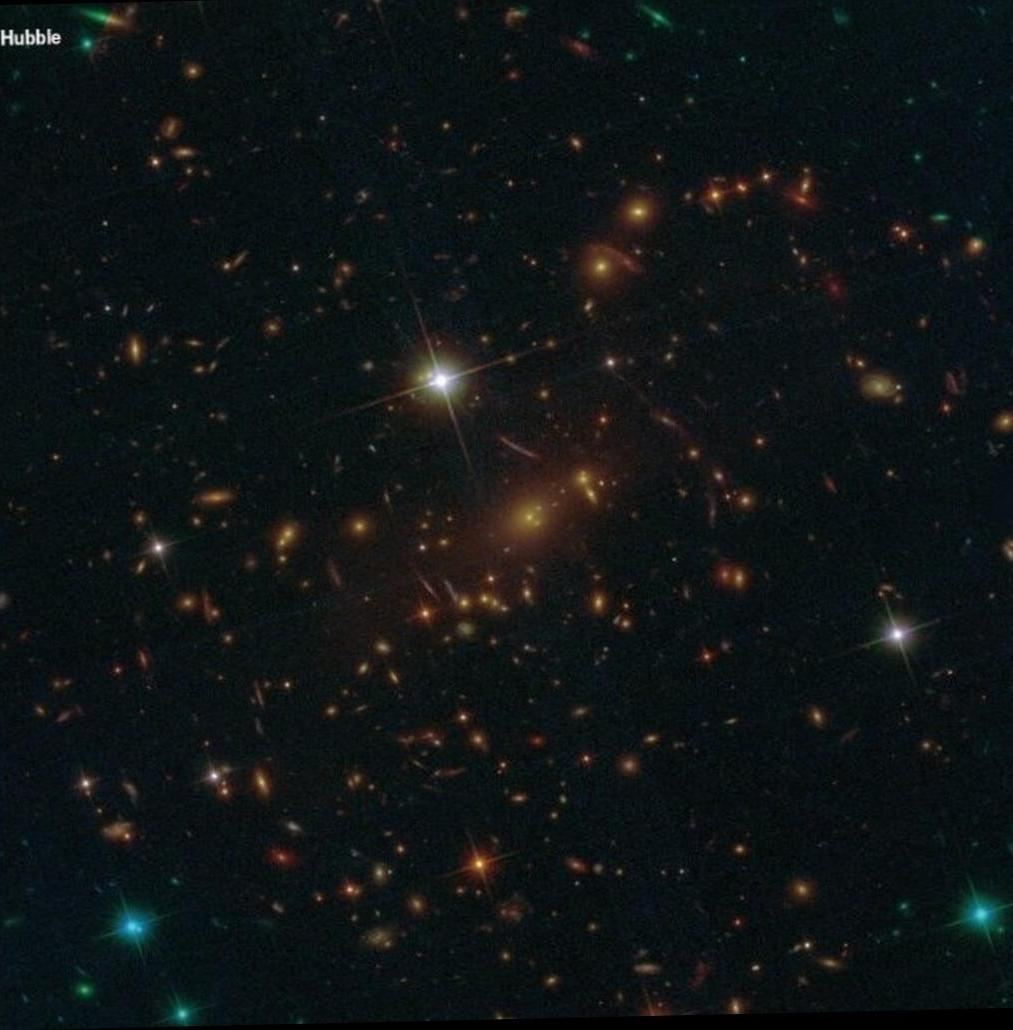
\includegraphics[width=0.8\textwidth]{hubble-deep-field.jpg}
\EC
}

\frame{\frametitle{\bf The problem with the {\color{orange} hot new thing}}

\BC
\Large Everything with a temperature produces light.\\ This is called {\it thermal radiation} or {\it blackbody radiation}.
\EC
\BS

\BCC
\small
\color{green}
\HC
Hotter objects produce shorter wavelengths:
\BI
\color{green}
\item Stars like the Sun: thousands of Kelvin, wavelengths around 500 nm (visible)
\item Hotter stars: tens of thousands of Kelvin, mostly ultraviolet
\EI
\pause
\BS
\color{orange}
Cooler objects produce longer wavelengths: 
\BI
\color{orange}
\item Earth-temperature things: hundreds of Kelvin, wavelengths around 10,000 nm
\item This is the famous ``heat vision'' -- it's not heat, it's just long-wavelength light
\EI

\normalsize \color{yellow}

... but redshifted, distant hot objects produce the same wavelengths as nearby cool ones!
\HC
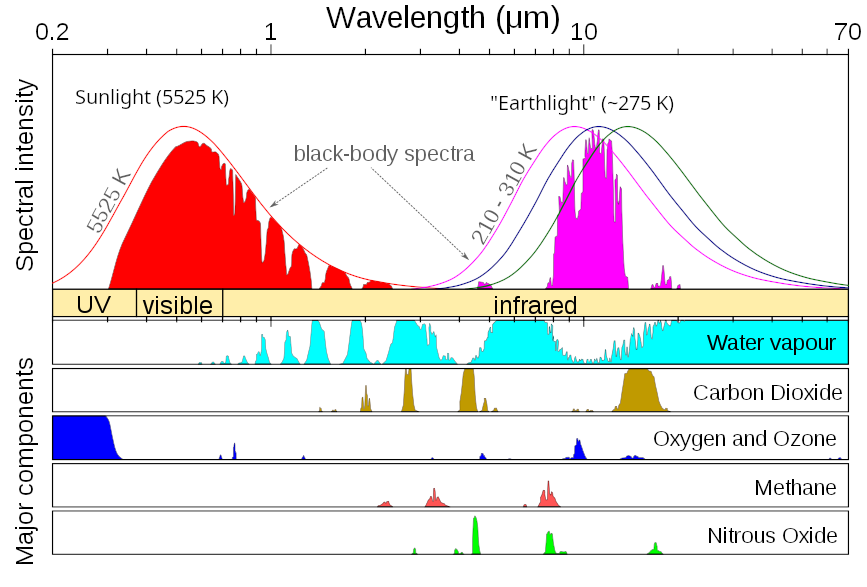
\includegraphics[width=\textwidth]{atmosphere-4.png}
\ECC
\large\pause
\BS
\BC
\color{red} Hubble is blinded by its own thermal radiation when trying to see the early universe!
\EC


}
	
\frame{\frametitle{\bf The Webb Space Telescope}

\BC
\Large		
Goal: Make highly detail observations from the visible to the infrared.
\EC

\BCC

\HC

\BI
\item Put it in space (no pesky air)
\BS
\item Make it big 
\BI
\item Earth-based telescopes now use honeycomb mirrors for easier manufacturing
\item NASA had to figure out how to fold one up
\item ... and unfold it in space without breaking it
\EI
\BS
\item Keep it in the shade so it's cool
\BI
\item The Earth and Moon produce infrared, so we have to shade it from them as well
\item It's parked in an orbit so that the Earth, Moon, and Sun are always on the same side
\EI
\EI

\HC
\BC
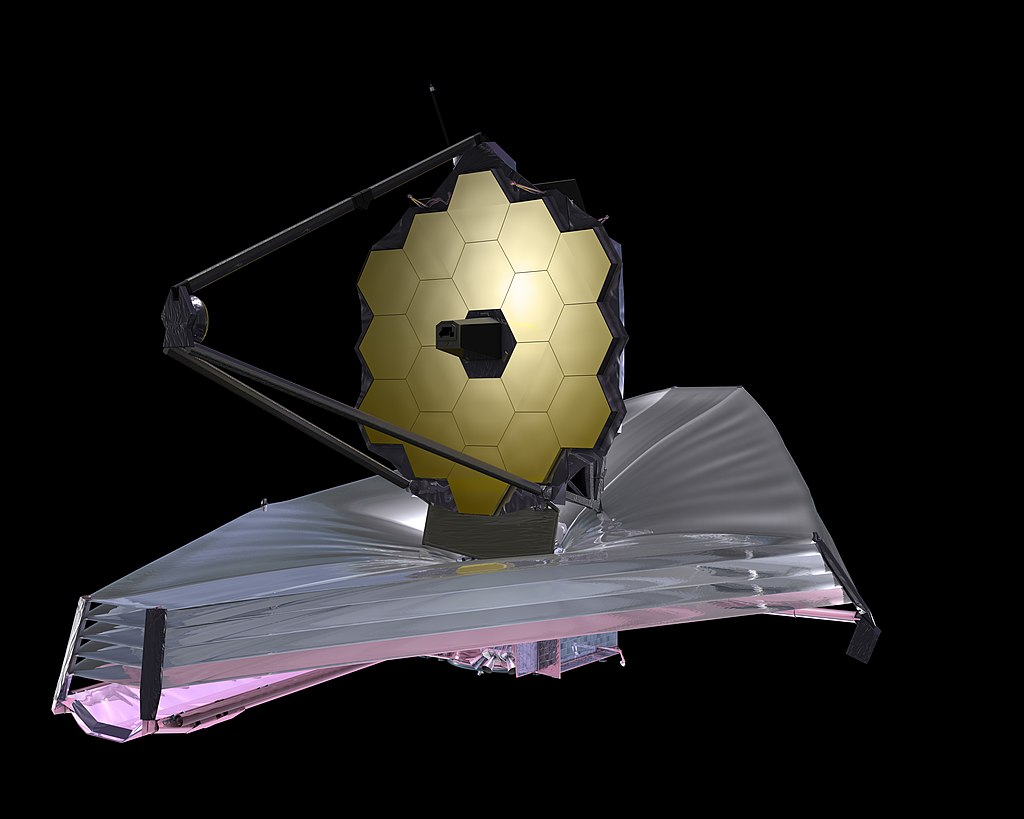
\includegraphics[width=0.9\textwidth]{jwst.jpg}
\scriptsize \\
Illustration of JWST. We didn't unfold it on the ground\\
and it doesn't have a selfie camera. :(
\EC
\ECC

}
\frame{
	\begin{center}
	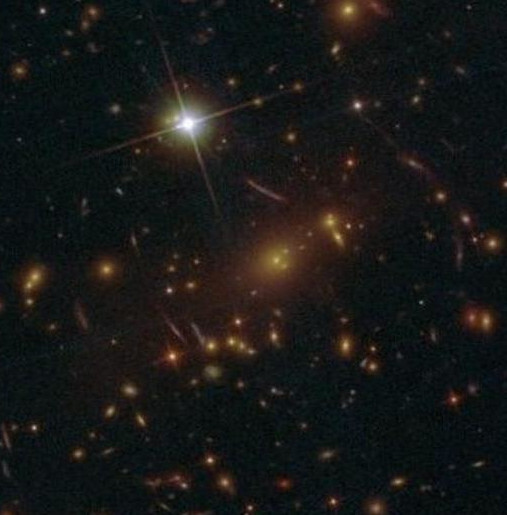
\includegraphics[height=0.9\textheight]{hubble-deep-field-crop.jpg}\\
	\scriptsize Hubble Space Telescope deep field (NASA)
	\end{center}
}

\frame{
	\BC
	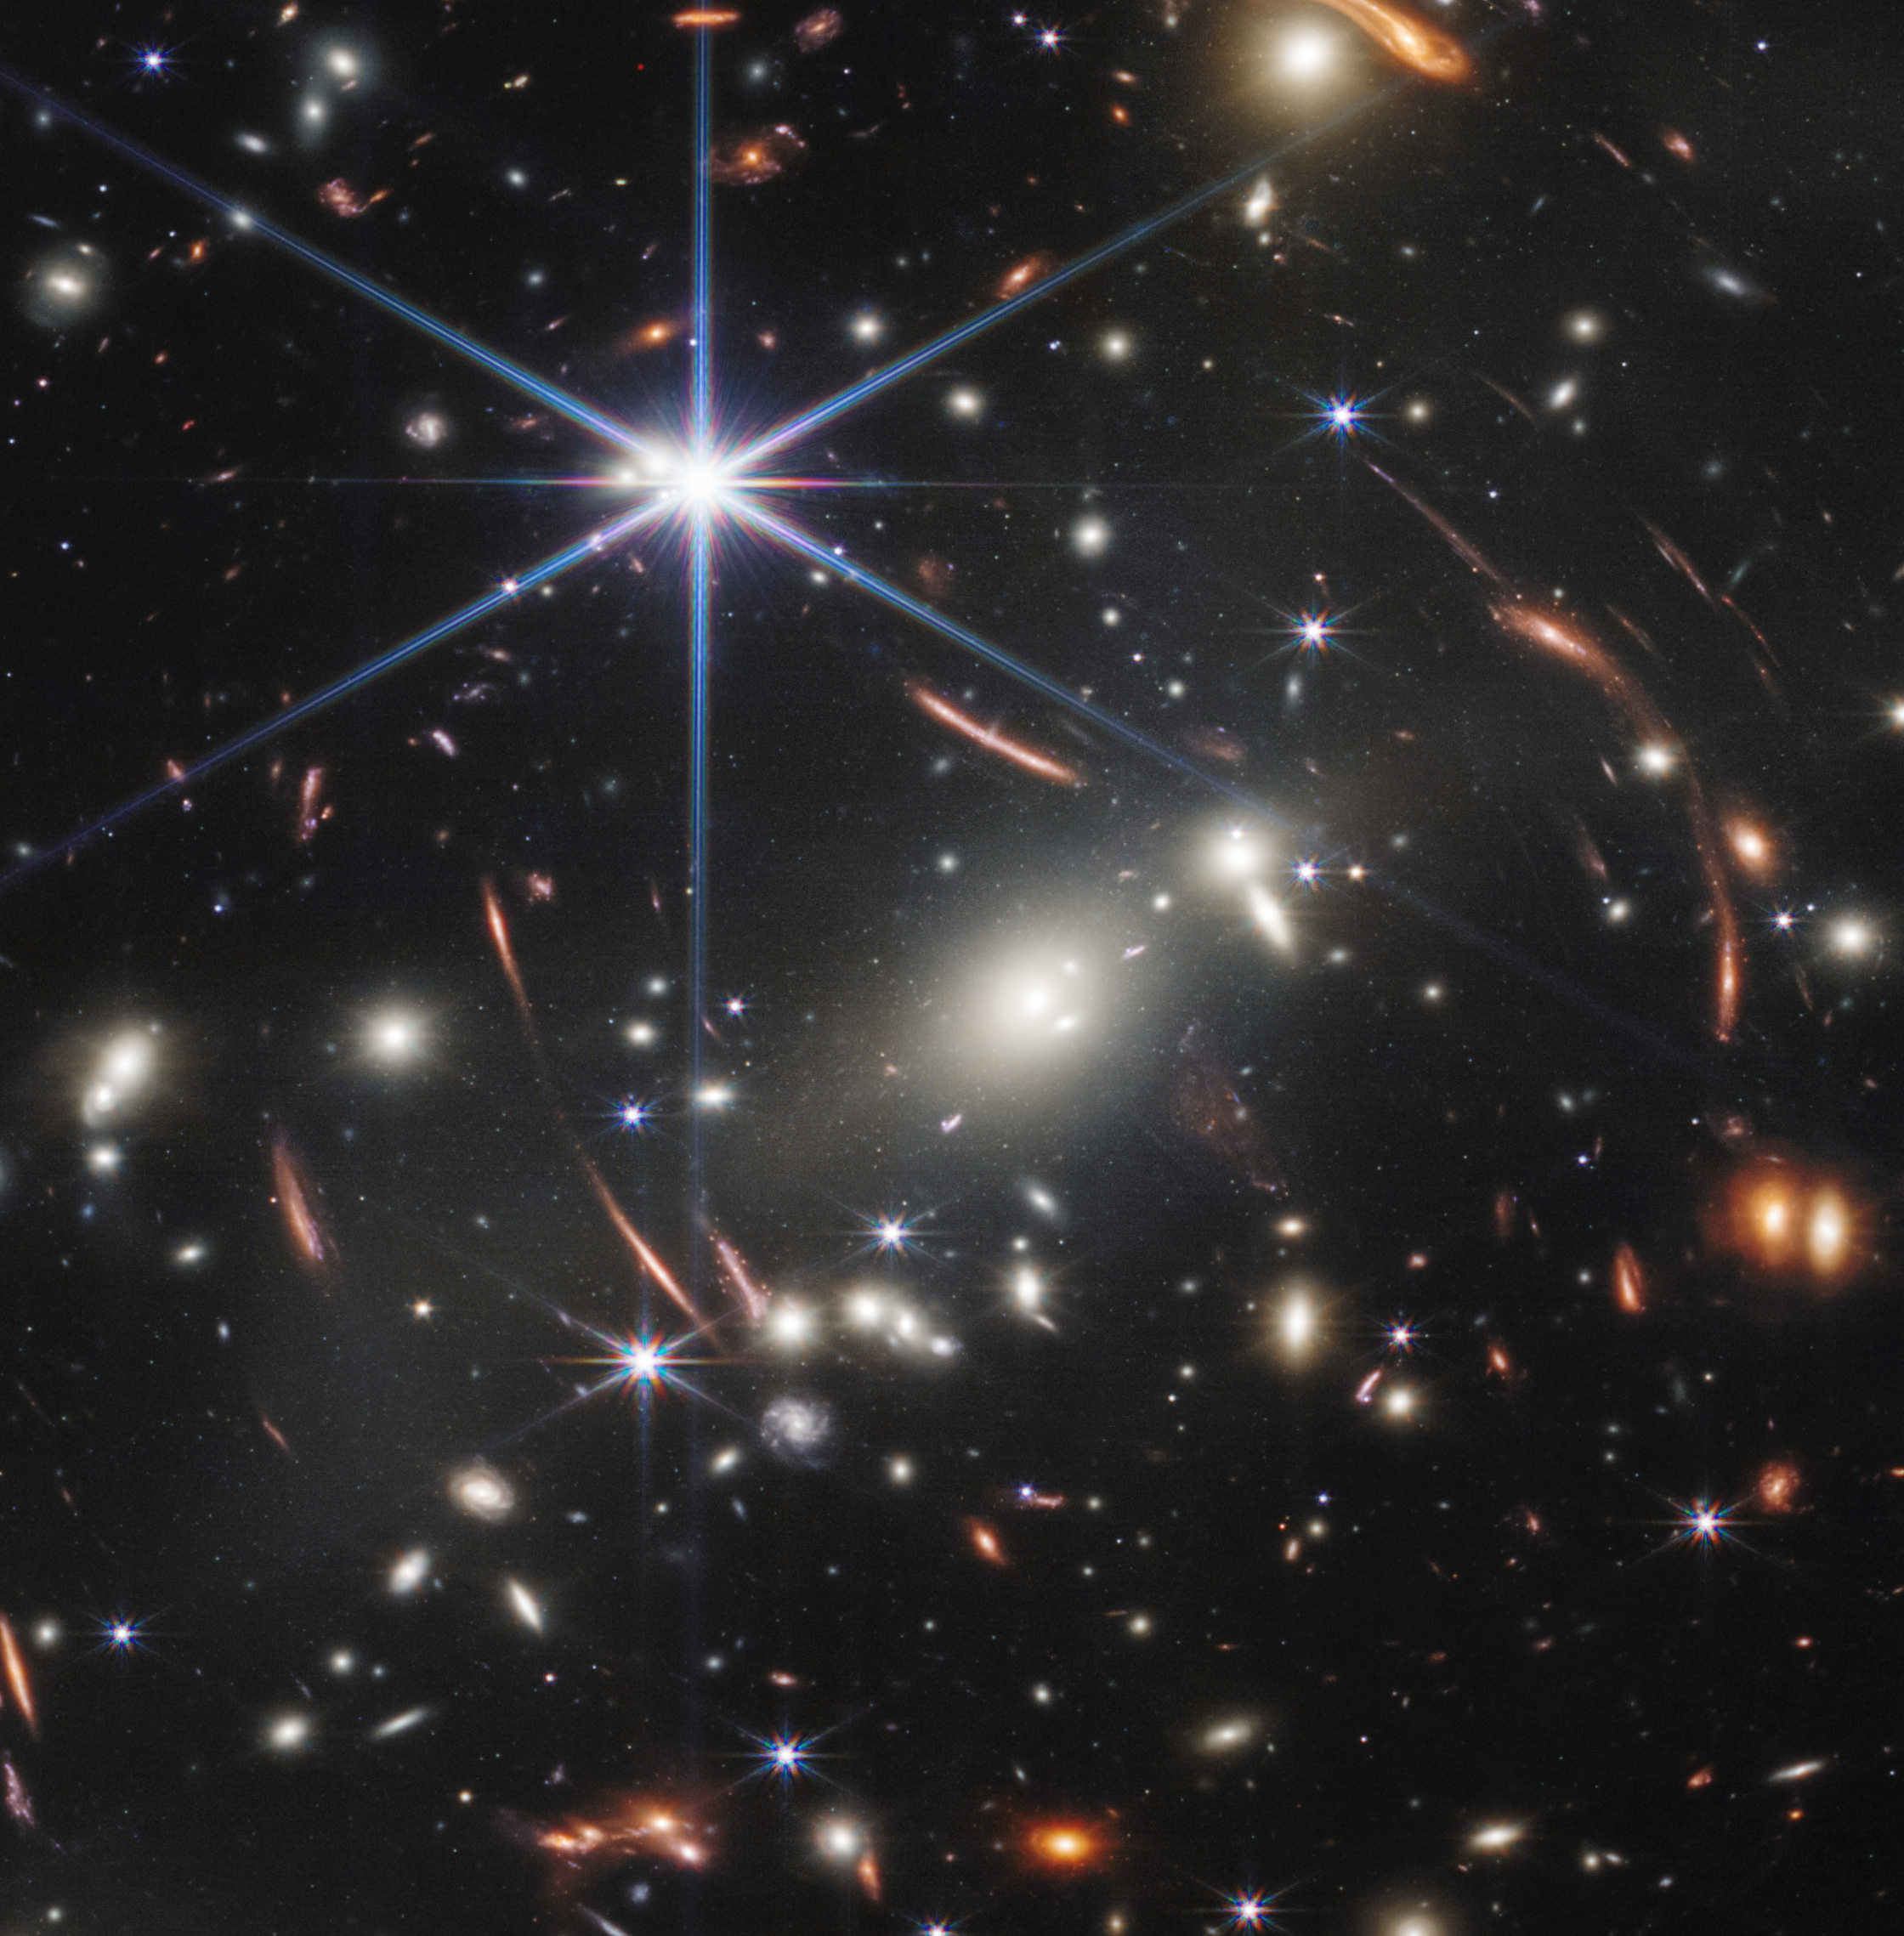
\includegraphics[height=0.9\textheight]{jwst-deep-field-crop.jpg}\\
	\scriptsize JWST deep field (near-infrared, similar to visible light) 
	\EC
}
			
\frame{
	\BC
	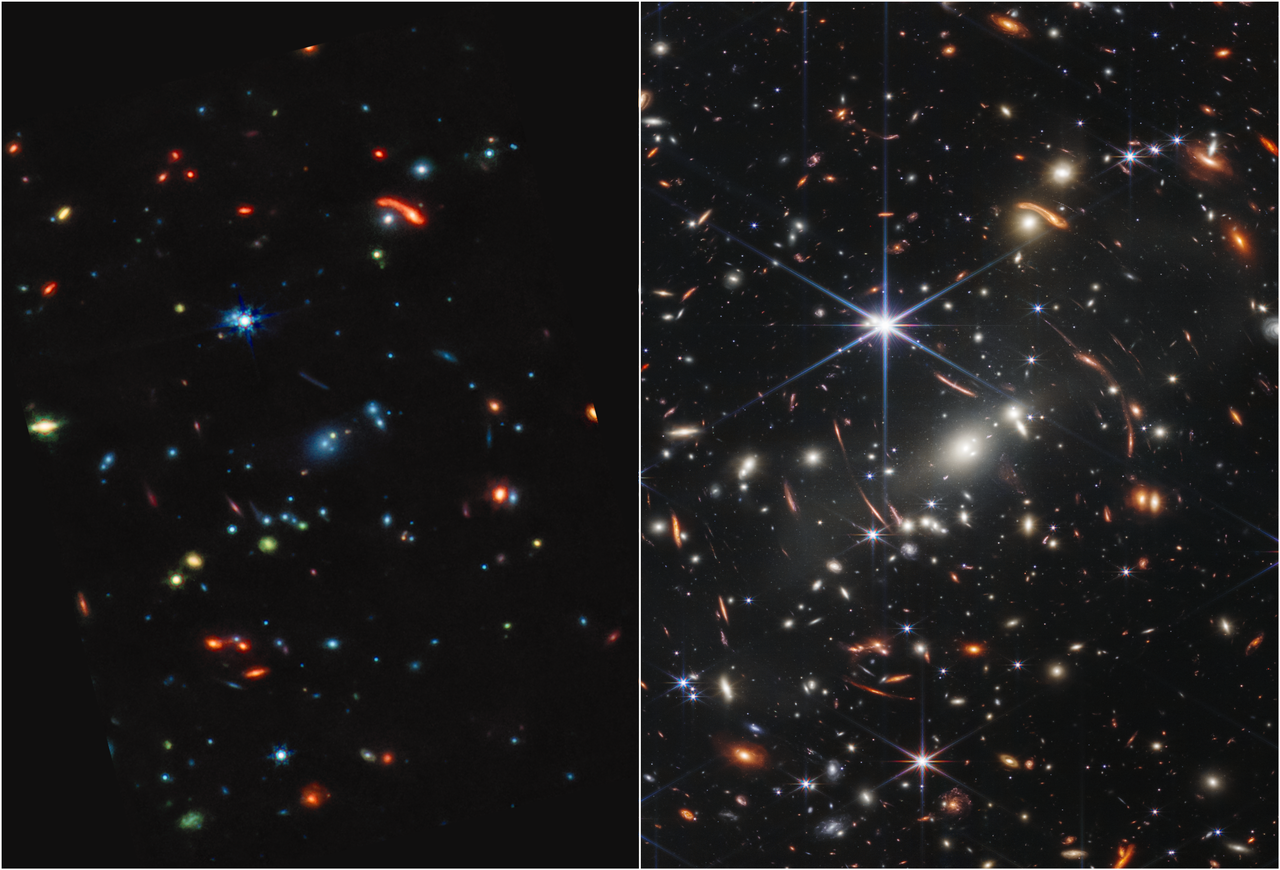
\includegraphics[height=0.9\textheight]{deep-field-side-by-side.png}\\
	\scriptsize JWST deep field: far infrared on left, near infrared on right
	
	\EC
}	

\frame{
	\BC
	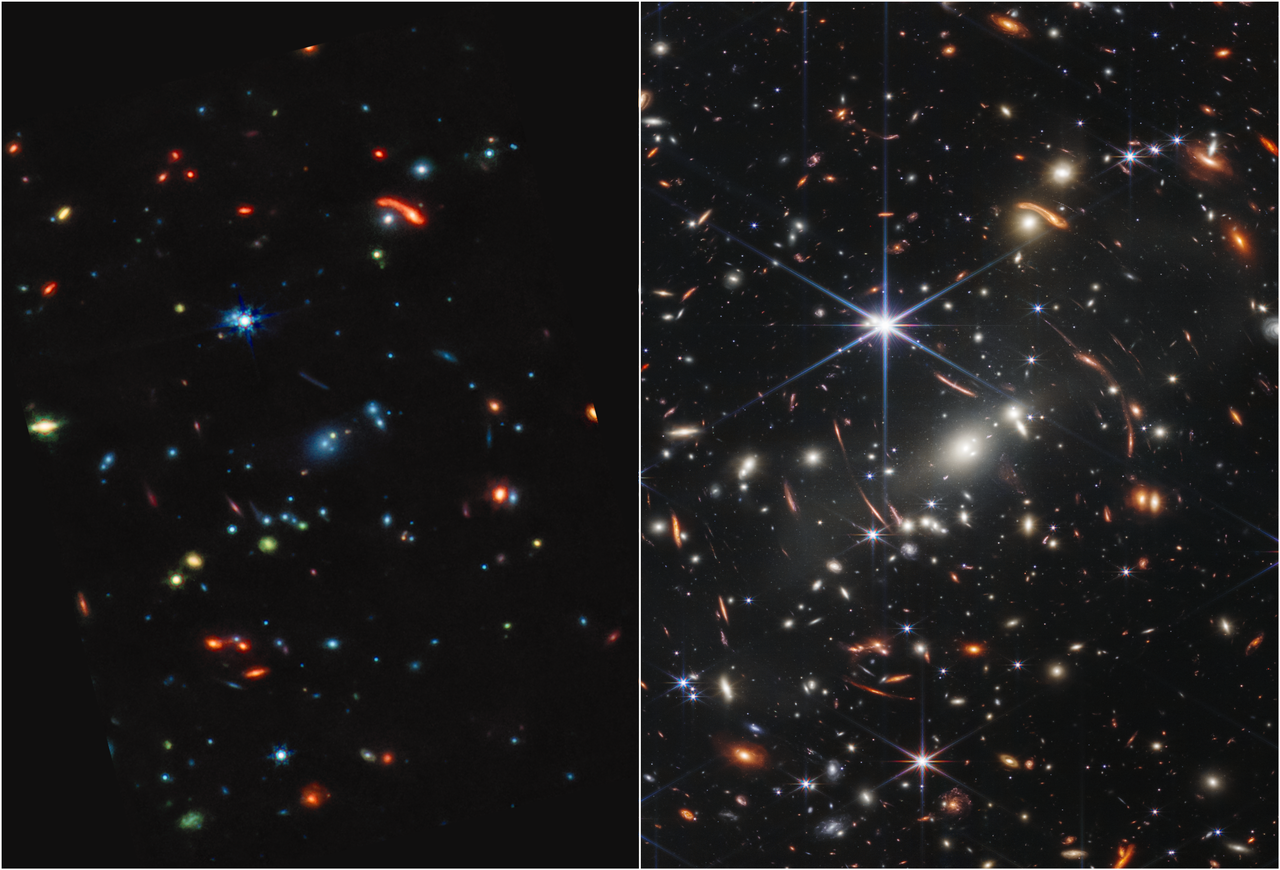
\includegraphics[height=0.9\textheight]{deep-field-side-by-side.png}\\
	\scriptsize JWST deep field: far infrared on left, near infrared on right
	
	\EC
}	

\frame{
	\BC
	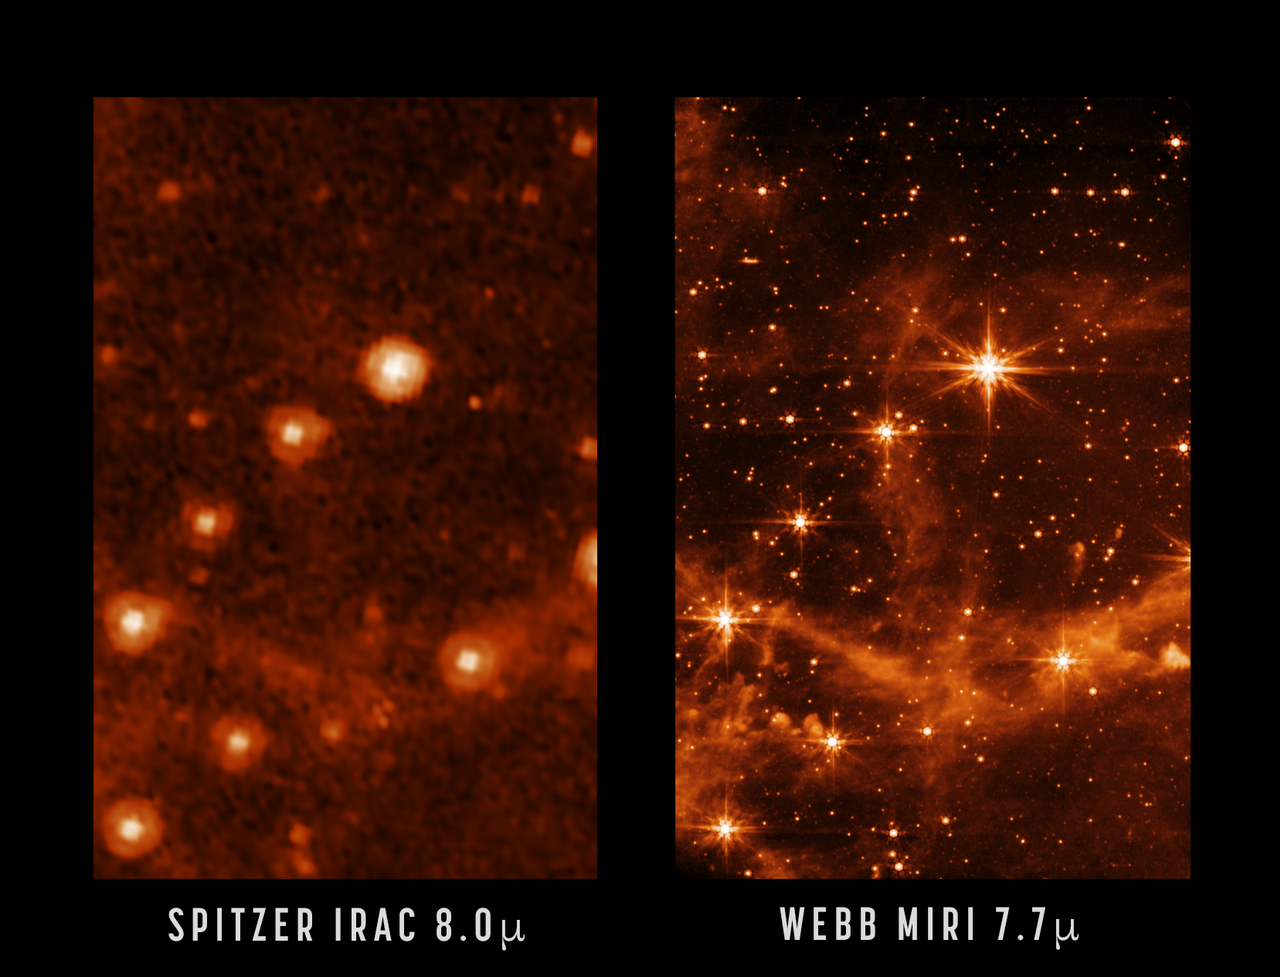
\includegraphics[height=0.9\textheight]{miri-test.png}\\
	\scriptsize Comparison between JWST and Spitzer Space Telescope 
	
	\EC
}	

\frame{
	\BC
	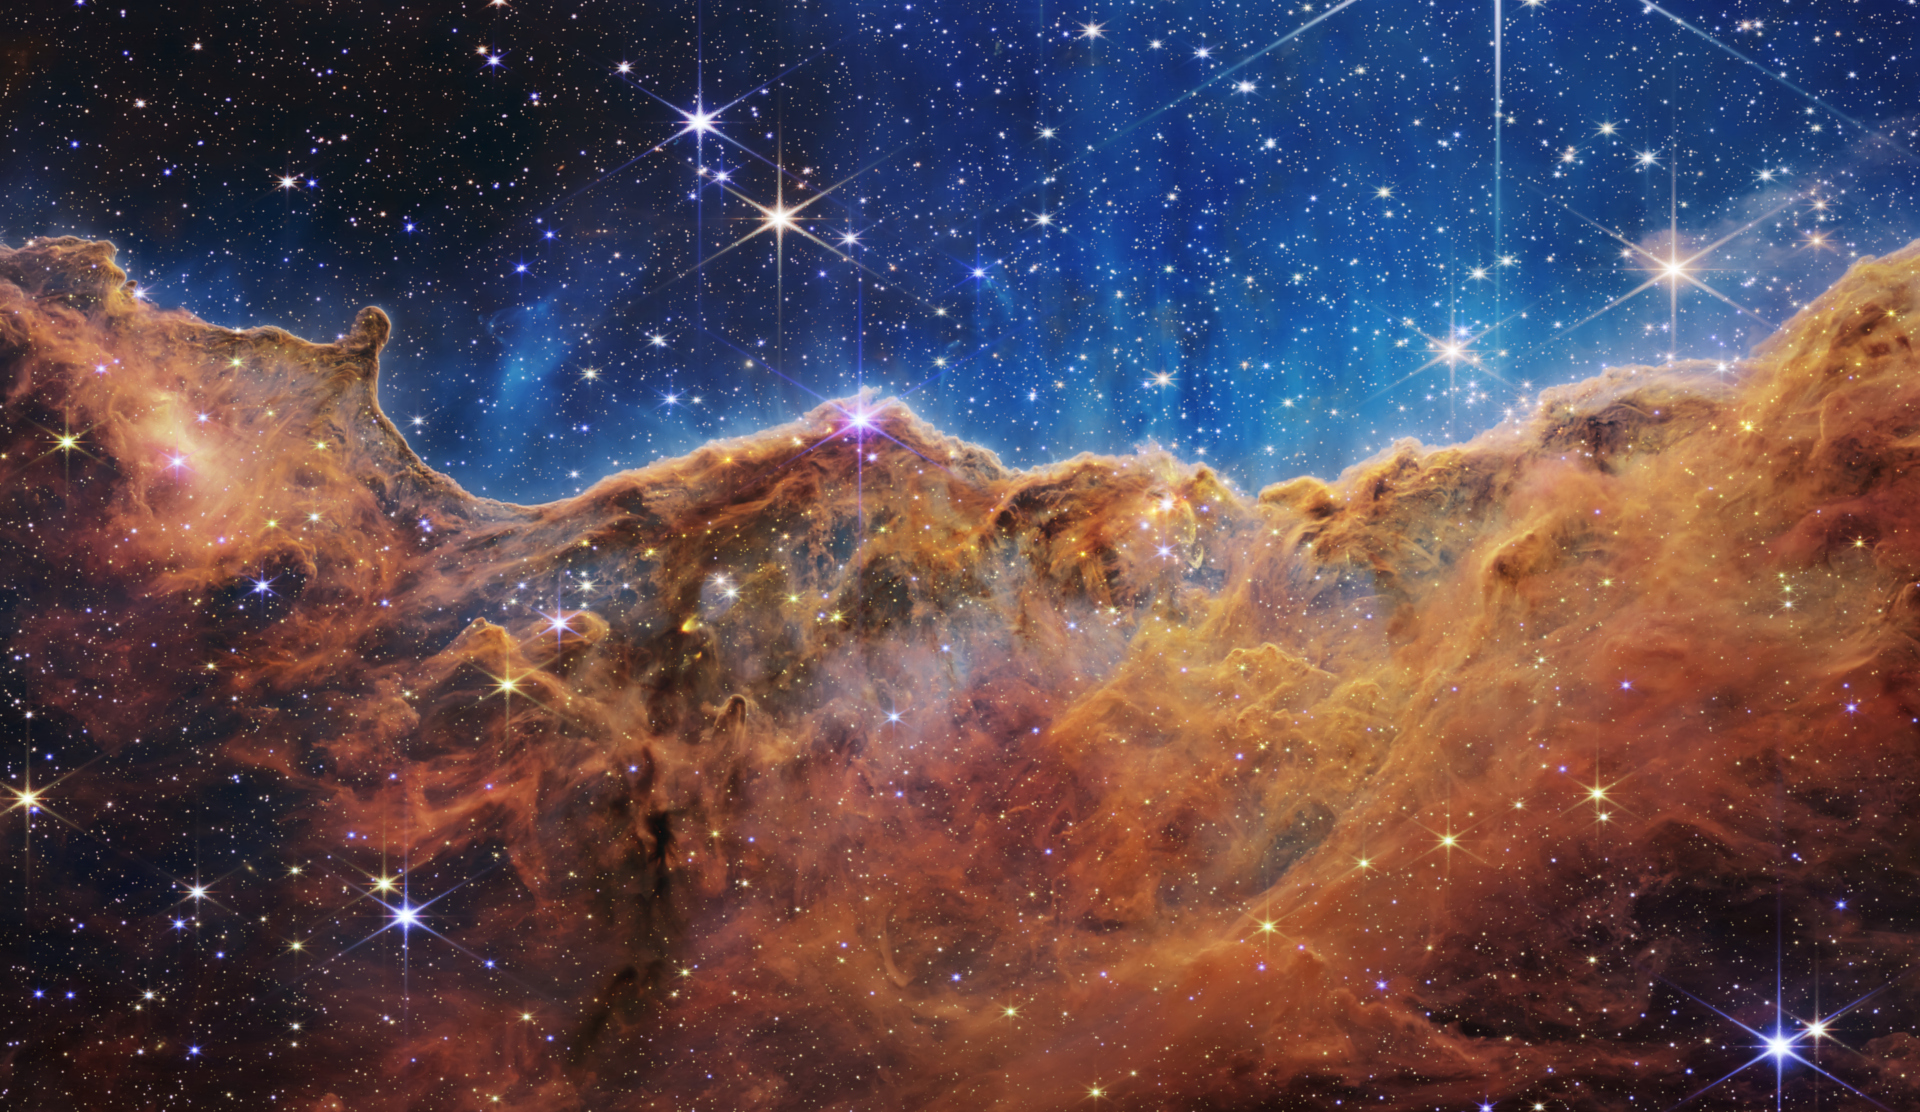
\includegraphics[height=0.85\textheight]{cosmic-cliffs.jpg}\\
	\small The ``cosmic cliffs'' in Carina Nebula, an active star-forming region\\ (near-infrared image by JWST)
	
	\EC
}	

\frame{\frametitle{\textbf{Planetary science with JWST, too}}
	\BC
		Water absorbs known wavelength bands in the infrared. We've seen its signature elsewhere in our Solar System.
		What about in planets around other stars? This is really hard. Can JWST do it?
		\EC
	\BCC
	\HC
	

	
	\BI
	\item Image a nearby star known to have a planet
 	\item Wait for a planet to pass in front of it
 	\item All wavelengths will be blocked equally by the planet
 	\item ... but the atmosphere will absorb {\it extra}
 	\EI
 	\HC
 	\BC
 	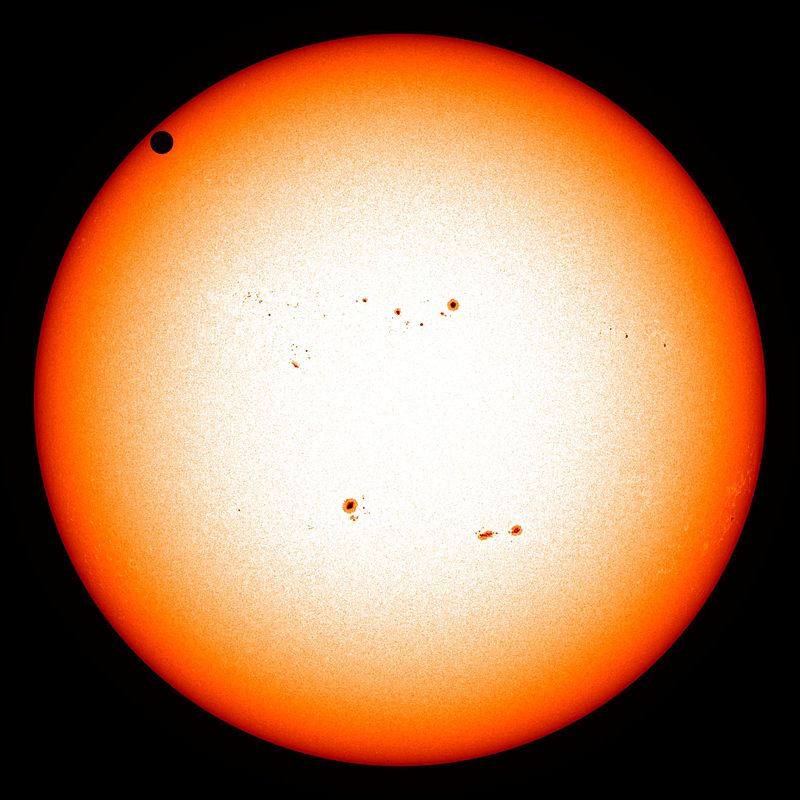
\includegraphics[width=0.65\textwidth]{transit-of-venus.jpg}
\\
\scriptsize Transit of Venus past the Sun, imaged by NASA's Solar Dynamics Observatory in 2012
 	\EC
 	\ECC
 	
 }
\frame{
\BC
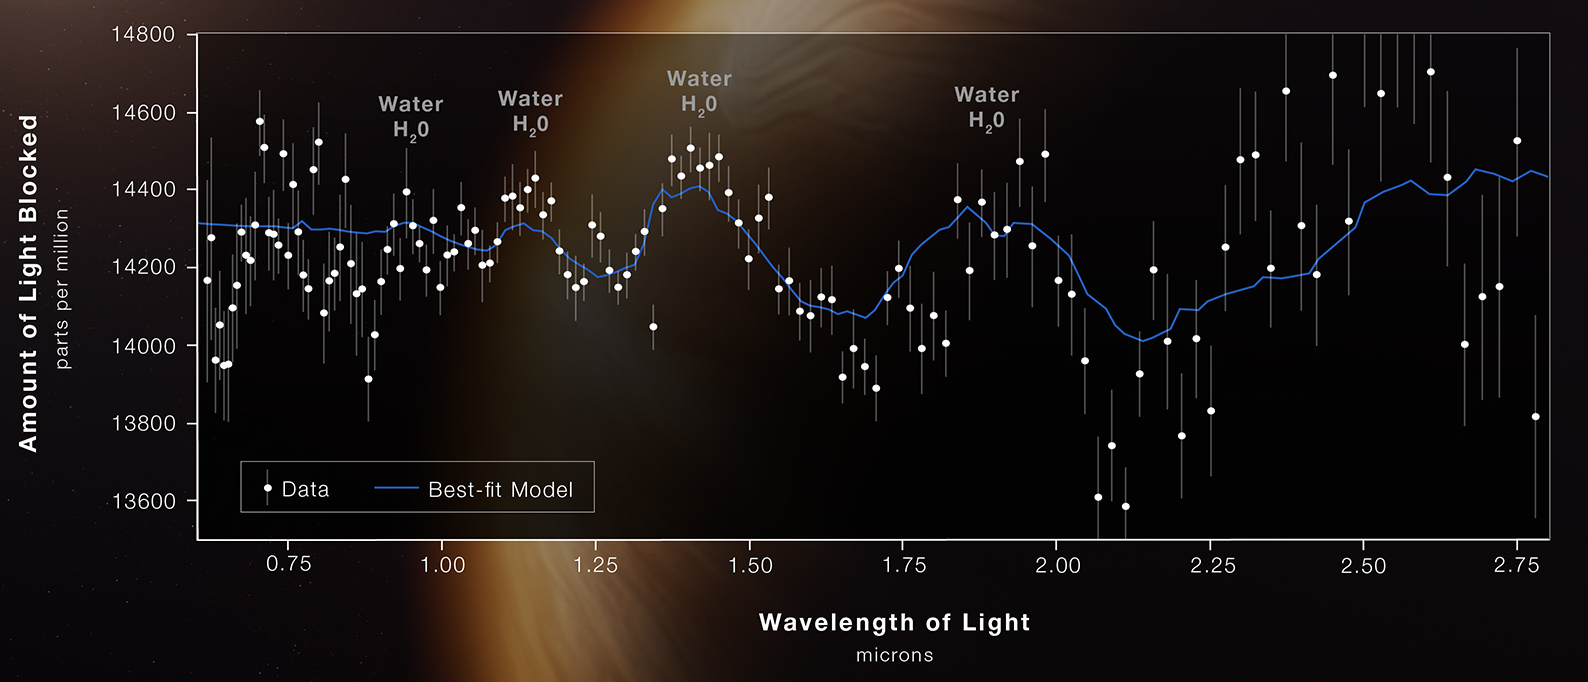
\includegraphics[width=0.95\textwidth]{wasp-exoplanet.jpg}
{\it \scriptsize Data and presentation from NASA}


\BS

JWST has seen the signature of water in another solar system!

\EC
}

\frame{
\BC
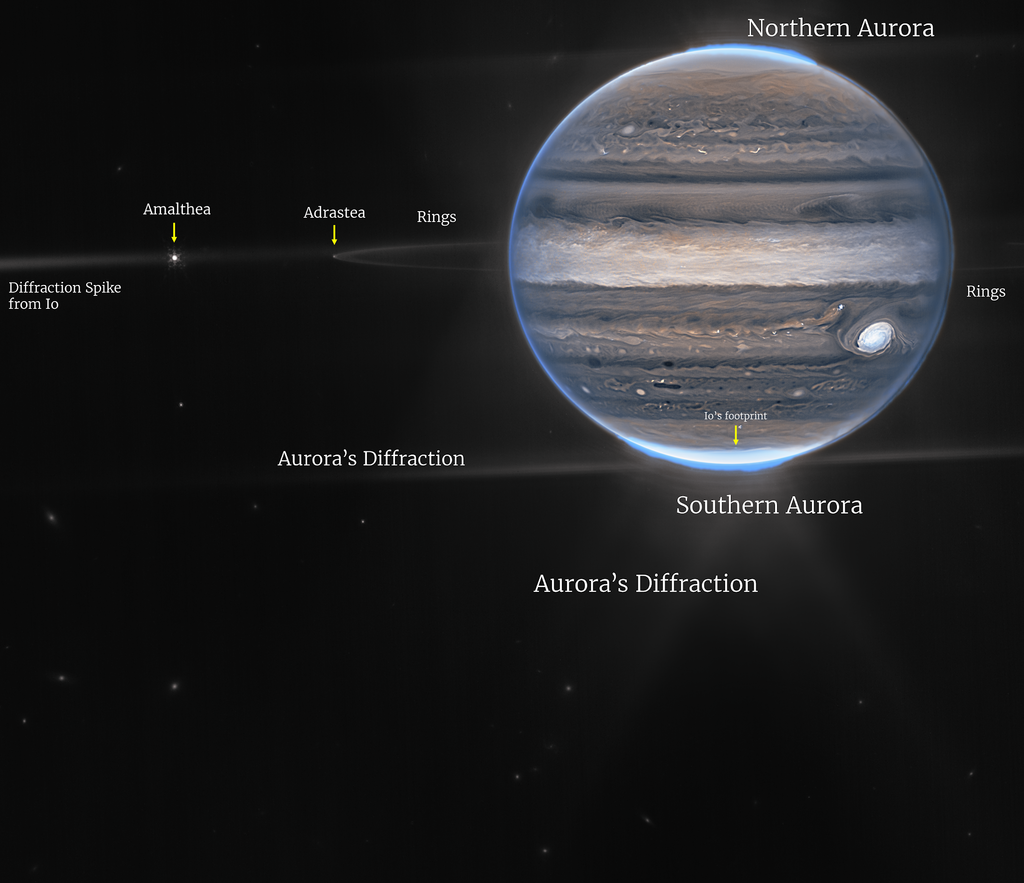
\includegraphics[width=0.95\textwidth]{jupiter.png}
\BS
... and the auroras on Jupiter! (Image and annotation from NASA)
\EC
}

\frame{
\BC
Thanks for coming -- please ask questions!
\BS
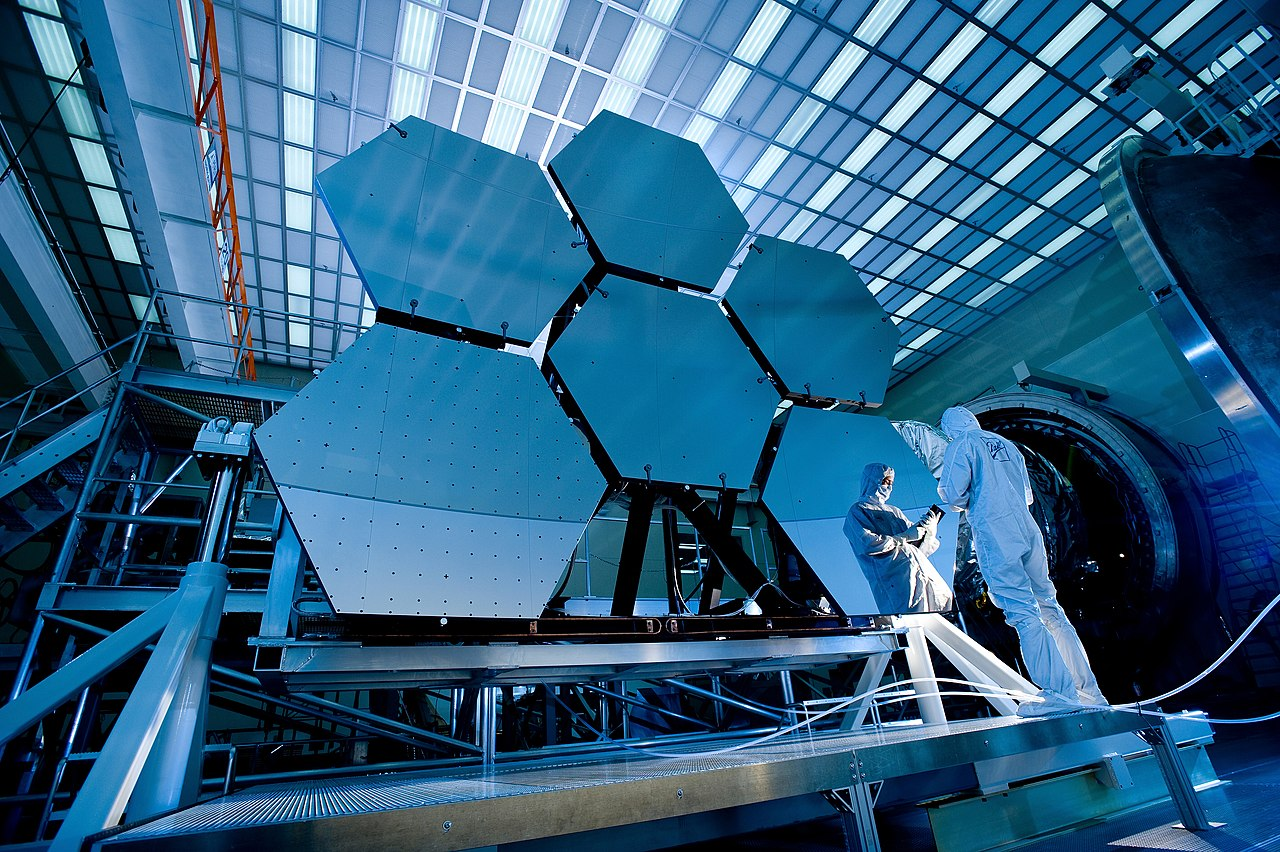
\includegraphics[width=0.7\textwidth]{jwst-marshall.jpg}
\BS
\\
\it Testing of JWST mirror segments at ultracold temperatures at Marshall Space Flight Center,
in Huntsville, Alabama, my hometown. (Image from NASA.)

\EC

}

\end{document}


